\documentclass[12pt]{article}

% margins and page style
\usepackage[margin=2.5cm]{geometry}
\usepackage{fancyhdr}
\pagestyle{fancy} 

% spaces between paragraphs
\usepackage[parfill]{parskip}

% fonts
\usepackage[T1]{fontenc}
\usepackage[scaled=0.92]{helvet}
\renewcommand*\familydefault{\sfdefault}

% font size of section headings
\usepackage{sectsty}
\sectionfont{\fontsize{14}{15}\selectfont}

% tables 
\usepackage{booktabs}
\renewcommand{\arraystretch}{1.5}

% figures
\usepackage{graphicx}
\usepackage[font=small,labelfont=bf]{caption} 

% colors
\usepackage[dvipsnames,svgnames,hyperref,table]{xcolor}

% hyperlinks
\usepackage{hyperref}
\hypersetup{
  pdfauthor={Erin C. McKiernan},
  colorlinks=true,
  urlcolor=Bittersweet,
  linkcolor=blue,
  citecolor=Purple,
}

% bib options
\let\oldbibliography\thebibliography
\renewcommand{\thebibliography}[1]{\oldbibliography{#1}
\setlength{\itemsep}{0pt}} 
\usepackage[numbers,sort&compress]{natbib} 
\bibliographystyle{unsrtnat}

% title and authors
\title{\vspace{-1.8cm}\Large{\textbf{Investigating the biophysics of respiration using electromyography and spirometry}}}
\author{}
%\author[1, \email]{Erin C. McKiernan} 

%\affil[1]{\small{Departamento de F\'isica, Facultad de Ciencias, Universidad Nacional Aut\'onoma de M\'exico}}

%\affil[ \email]{\small{emckiernan@ciencias.unam.mx}}
\date{}

%%%%%%%%%%%%%%%%%%%%%%%%%%%%%%%%%%%%%%%%%%%%%%%%%%%%%%%%%%%%
 
\begin{document}
\maketitle


\section*{OVERVIEW}

In this laboratory practical, students will use a spirometer to record the volume of air inhaled and exhaled during normal and forced respiration while simultaneously recording electromyograms from different respiratory muscles. Overall, this practical will help students understand the mechanics of respiration, and comprehend the relationship between electrical activation of respiratory muscles and the volume of air inhaled or exhaled.

\section*{SPECIFICATIONS}
\begin{tabular}{p{6cm} p{10cm}}
\textbf{Level of study:} & Undergraduate \\
\textbf{Degree programs:} & Biology, Physics, Biomedical Physics, others \\
\textbf{Semester:} & 4th to 6th (i.e. 2nd to 3rd year undergrads) \\ 
\textbf{For use in courses:} & Systems Physiology, Physics of the Human Body, others \\
\textbf{Recommended prior courses:} & Molecular \& Cellular Biology \\
\textbf{Duration of practical:} & 2 hours \\
\textbf{Setting:} & Classroom or laboratory \\
\textbf{Safety considerations:} & Have chairs available for participants to sit in case repeated and forced breathing protocol causes lightheadedness; Use disposable filters and mouthpieces and disinfect spirometer between subjects to avoid passing germs. \\
\textbf{Other indications:} & Wear loose clothing to permit unhindered breathing and electrode placement
\end{tabular}

\section*{OBJECTIVES}
\textbf{Before doing this lab you should be able to:}
\begin{itemize}
\item describe the anatomy of the lungs and respiratory system
\item identify and locate the primary and accessory respiratory muscles 
\item explain how muscles contract and relax
\end{itemize}
 
\vspace{0.3cm}

\textbf{In this lab you will:}
\begin{itemize}
\item learn how to use a spirometer 
\item learn how to record electromyograms (EMGs)
\item observe and record changes in air volume when you inhale and exhale
\item observe and record the activation of different muscle groups during inhalation and exhalation
\item investigate how volumes and muscle activations differ between normal and forced respiration
\end{itemize}

\vspace{0.3cm}
 
\textbf{After doing this lab you should be able to:}
\begin{itemize}
\item understand the basic mechanics of respiration
\item describe the role of primary versus accessory muscles in respiration
\item explain how normal and forced respiration differ
\item explain the relationship between contraction of different muscles and volume changes
\item design further experiments to investigate how respiration changes under different conditions
\end{itemize}

\section*{EQUIPMENT}

\textbf{For spirometry:}
 \begin{itemize}
	\item Spirometer (e.g. Vernier model SPR-BTA)
   	\item Disposable bacterial filters (Vernier)	
	\item Disposable mouthpieces (Vernier)
    \item Nose clip (Vernier)
	\item LabQuest 2 standalone interface (Vernier)
    \item Computer with Logger Pro software (Vernier) installed to analyze data (optional), or
    \item Computer with Python installed to analyze data (optional)
    \item Cleaning solution (i.e. Lysol spray or wipes)
\end{itemize}

\vspace{0.3cm}

\textbf{For electromyography:}
 \begin{itemize}
	\item Muscle SpikerBox (Backyard Brains)
    \item 3 surface electrodes (Backyard Brains or other provider)
    \item orange cable with alligator clips to connect electrodes to SpikerBox (Backyard Brains)
    \item cable to connect SpikerBox to a computer, tablet, or smartphone (Backyard Brains)
 	\item tablet, computer, or smartphone with free Backyard Brains SpikeRecorder software installed
    %\item two timers to aid in synchronizing recordings (optional)
\end{itemize}


\section*{BACKGROUND}

\subsection*{Types of respiration}

Respiration can be divided into two types depending on the effort exerted and the muscles involved: (1) normal respiration (eupnea), which is carried out under resting conditions, and (2) forced respiration (hyperpnea), which occurs when the oxygen demand of the body increases, for example, during exercise \cite{openStax2016resp}. Normal inhalation is an active process during which primary inspiratory muscles (see below) activate. Normal exhalation is a passive process during which the lungs return to their resting position due to elastic recoil. Forced inhalation involves extra effort to bring more than the normal volume of air into the lungs, and requires the activation of additional muscle groups. Forced exhalation, unlike normal exhalation, is an active process which requires the activation of select muscles to compress the thoracic cavity and lungs beyond the point of normal elastic recoil and push additional air out of the lungs \cite{openStax2016resp}.

\subsection*{Respiratory muscles and the mechanics of respiration}

The muscles involved in respiration can be classified as either primary or accessory, depending on whether they are activated during normal or forced respiration, respectively \cite{sieck2013mechanical}. 

\subsubsection*{Primary respiratory muscles}

The primary inspiratory muscles are the diaphragm and the external intercostals (Fig \ref{fig:primary}) \cite{openStax2016resp}. The diaphragm contracts, moving downward to increase the volume of the thoracic cavity in the vertical axis \cite{guyton20006textbook}. The external intercostals contract, pulling the rib cage up and out to expand the thoracic cavity in the anterior to posterior axis. During exhalation, the diaphragm and the external intercostals simply relax, returning to their resting positions due to the elastic recoil properties of the lungs and decreasing the volume of the thoracic cavity \cite{guyton20006textbook}. Thus, normal inhalation is an active process that requires the activation of the diaphragm and external intercostals, while normal exhalation is a passive process that involves muscle relaxation and elastic recoil of the lungs \cite{openStax2016resp}.

\begin{figure}[h!]
\centering
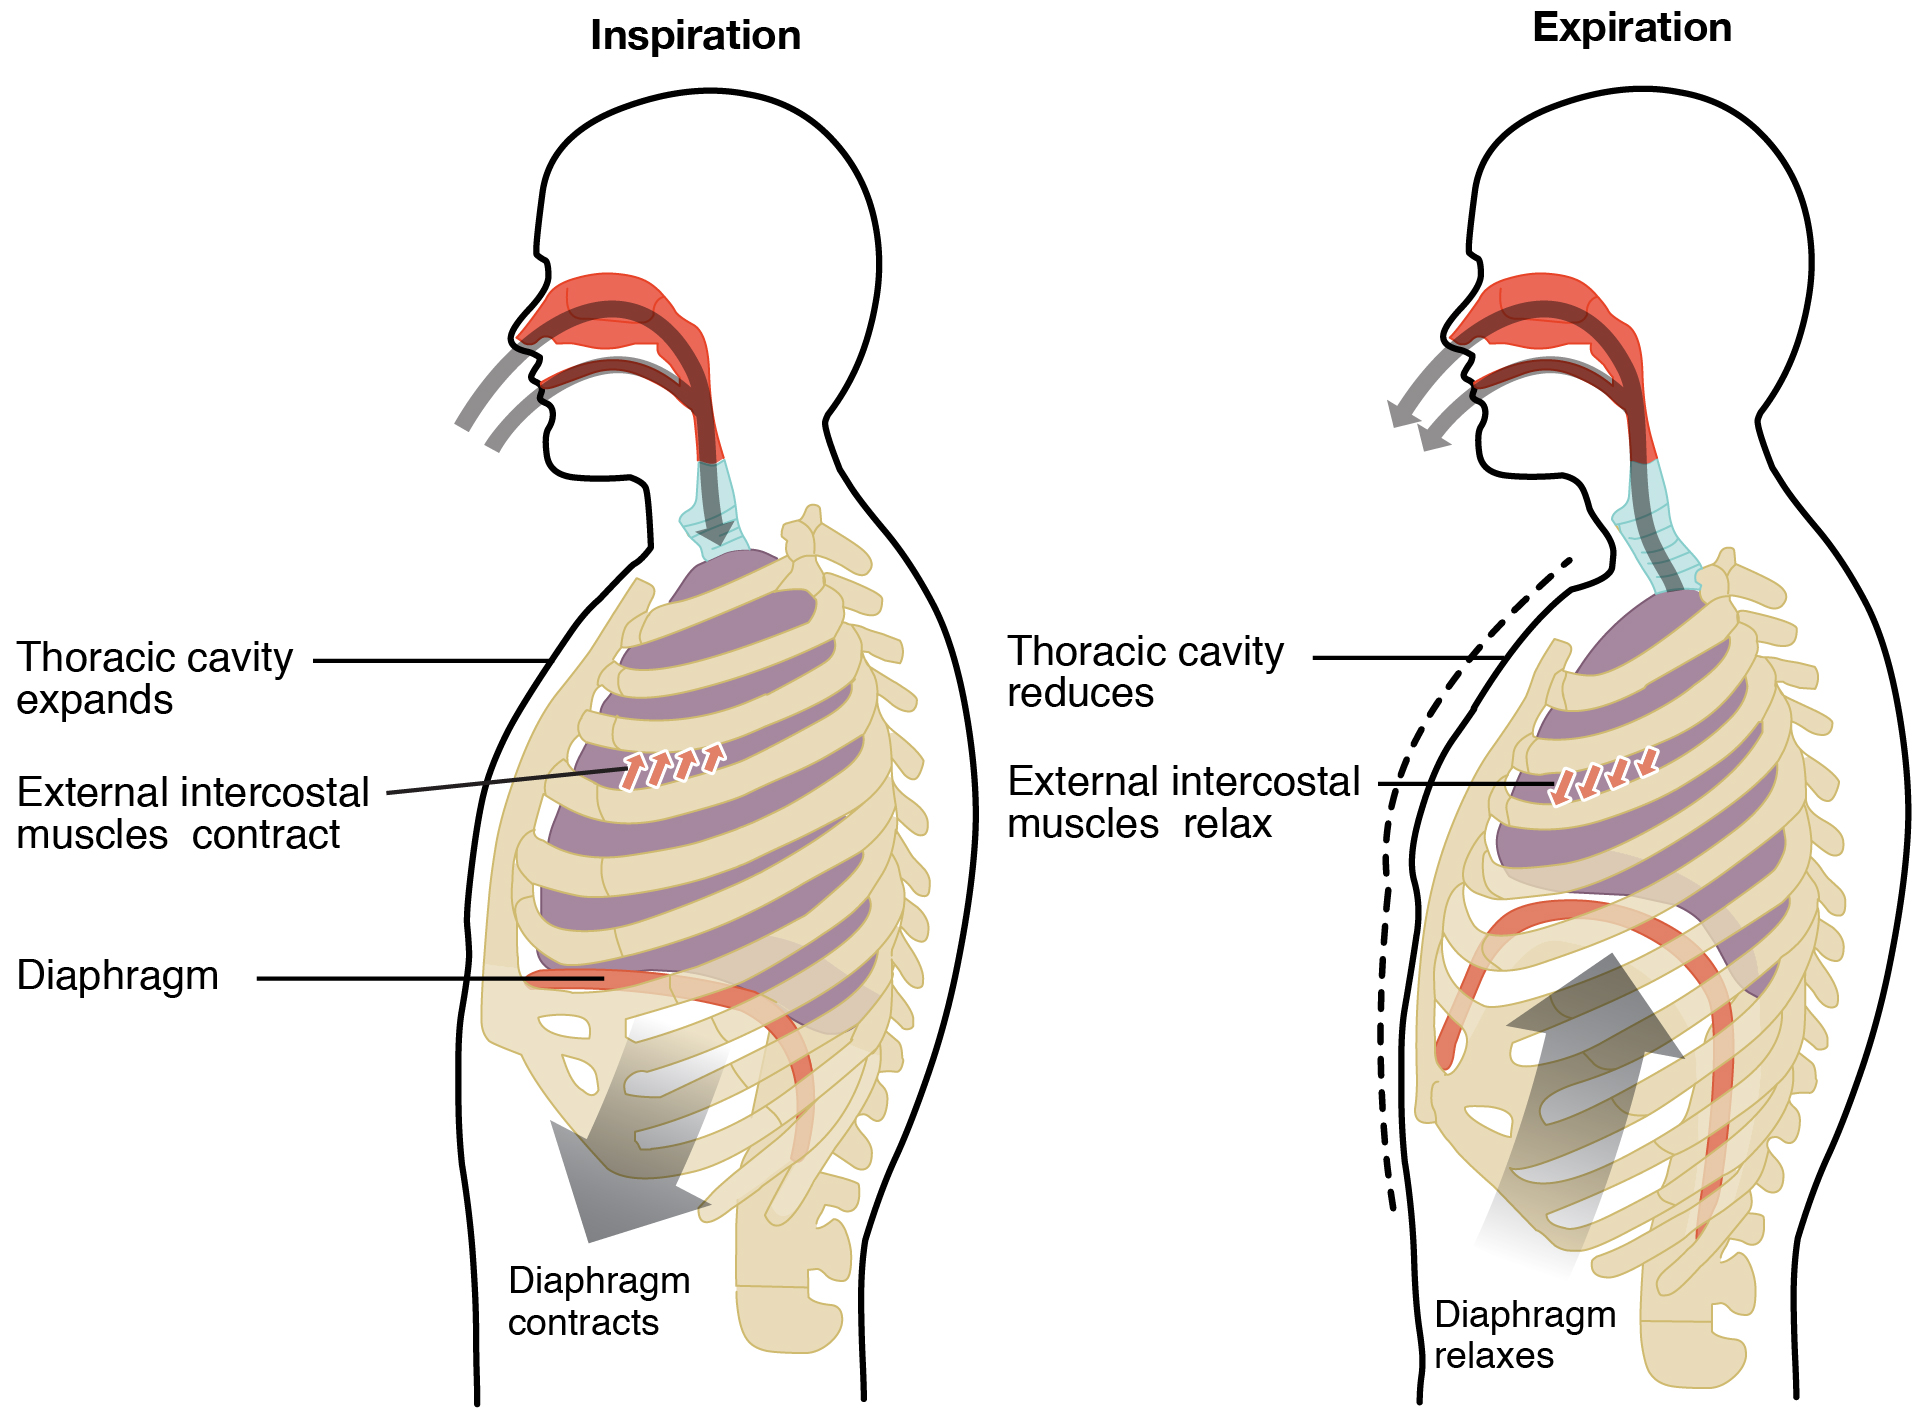
\includegraphics[width=0.7\textwidth]{images/Inspiration_and_Expiration.jpg}
\caption{Movement of the diaphragm and external intercostal muscles during normal inspiration and expiration. Image credit: OpenStax CNX \cite{openStax2016resp}, Creative Commons Attribution license (CC BY).}
\label{fig:primary}
\end{figure}

\subsubsection*{Accessory respiratory muscles}

The accessory muscles are those that only activate during forced respiration, when extra effort is required to pull more air in or push more air out of the lungs \cite{openStax2016resp,sieck2013mechanical}. The accessory muscles involved in forced inhalation are shown in Fig. \ref{fig:acc_insp} and include the sternocleidomastoid, the scalenes, the serratus anterior, and the pectoralis minor, among others \cite{troyer1986action,ratnovsky2008mechanics}. These muscles, found in the neck and chest areas, act to expand the volume of the thoracic cavity beyond what can be achieved by the primary inspiratory muscles alone and bring more air in. The accessory muscles involved in forced expiration are shown in Fig. \ref{fig:acc_exp} and include the internal intercostals, traversus thoracis, external oblique, internal oblique, and the rectus abdominus \cite{troyer1986action,ratnovsky2008mechanics}. These muscles, located in the chest and abdominal areas, act to further reduce the volume of the thoracic cavity and push more air out of the lungs than what can be achieved by simple elastic recoil.

\begin{figure}[h!]
\centering
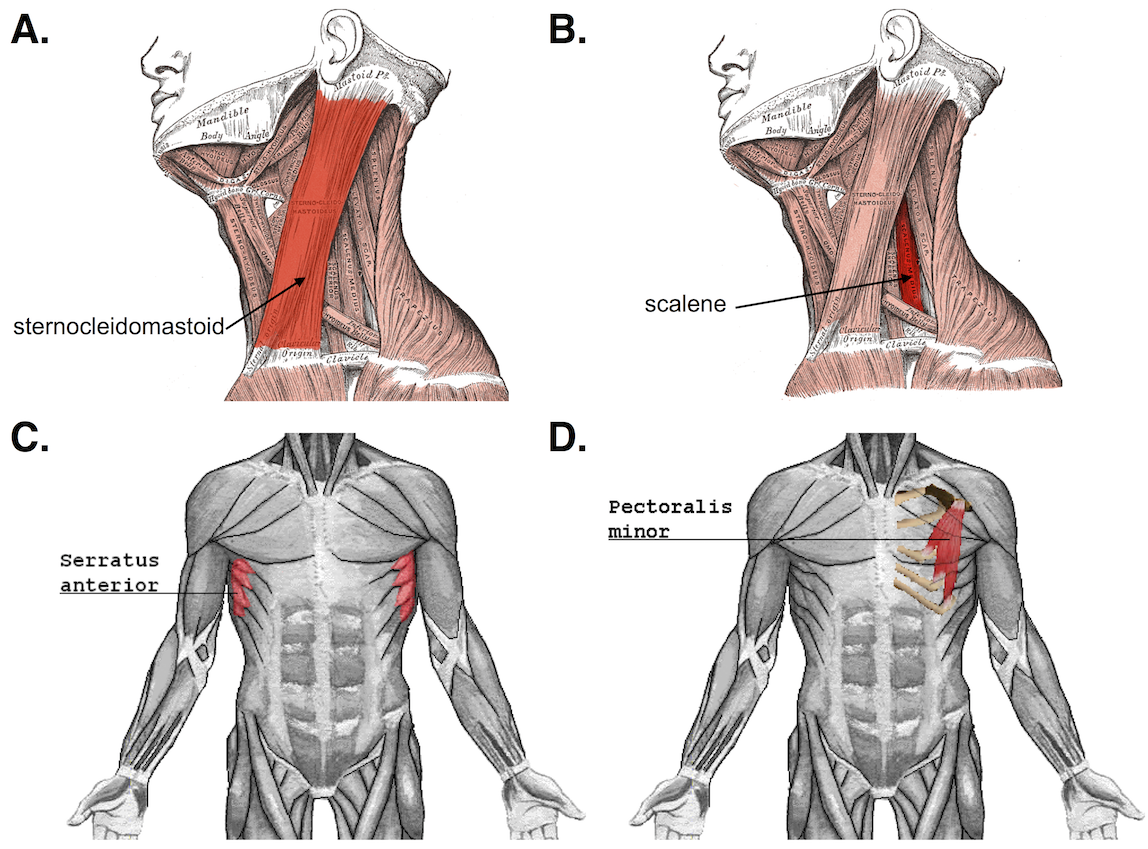
\includegraphics[width=0.75\textwidth]{images/accessory_insp.png}
\caption{Accessory inspiratory muscles. Image credits: A.,B. highlighted images from Gray's Anatomy (1858), public domain; C.,D. Originals by sv:Anv\"andare:Chrizz via Wikimedia Commons, Creative Commons Attribution-ShareAlike license (CC BY-SA).}
\label{fig:acc_insp}
\end{figure}%

\begin{figure}[h!]
\centering
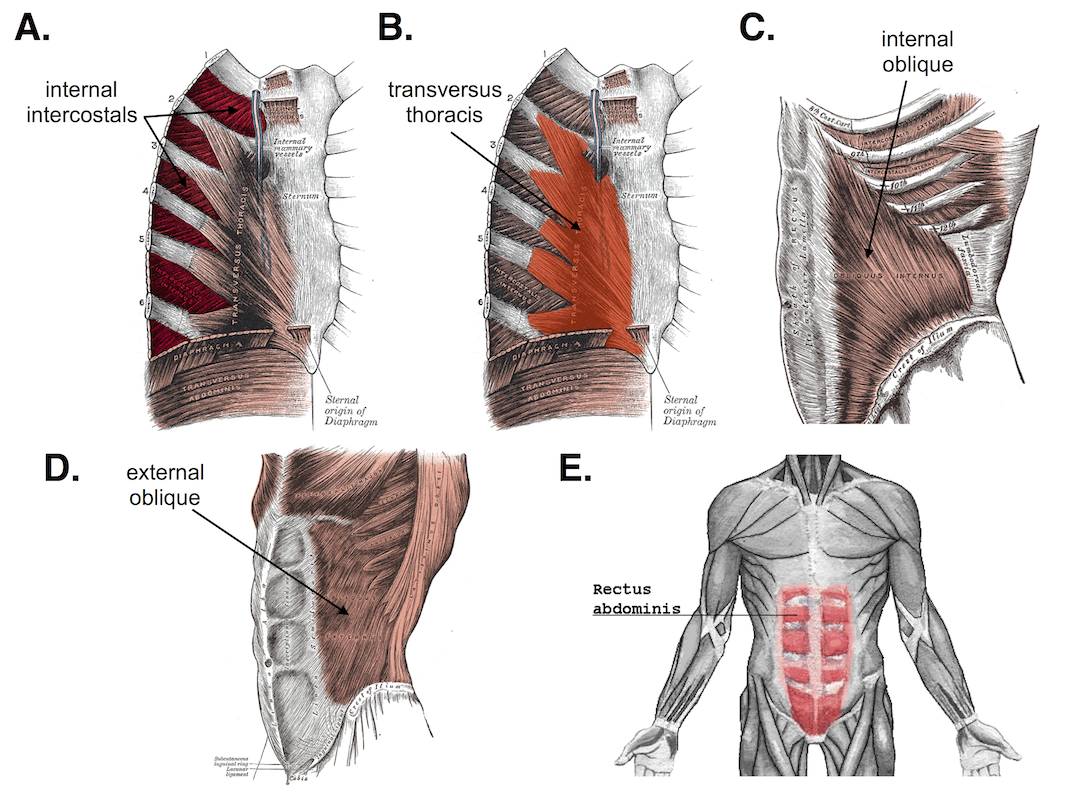
\includegraphics[width=0.76\textwidth]{images/accessory_exp.png}
\caption{Accessory expiratory muscles. Image credits: A-D. highlighted images from Gray's Anatomy (1858), public domain; E. Original by sv:Anv\"andare:Chrizz via Wikimedia Commons, CC BY-SA.}
\label{fig:acc_exp}
\end{figure}

\subsection*{Measuring the activity of respiratory muscles - electromyogram}

Muscles are composed of excitable cells which generate electrical impulses, called action potentials (APs). AP firing initiates cascades of cellular signaling events that eventually lead to muscle contraction. (For review of muscle physiology and excitation-contraction coupling, see Ch. 6-7 in \cite{guyton20006textbook} and also \cite{sieck2013mechanical}.) Thus, electrical activity in muscles is coupled to contractile activity. 

To record the electrical activity of muscles we use a technique called electromyography, and the recordings we obtain are called electromyograms (EMGs) \cite{garcia2011surface}. EMG recording can be done invasively by inserting electrodes into the muscle of interest, or non-invasively by using surface electrodes placed on the skin above the muscle (Fig. \ref{fig:emg}). Electrode insertion has the advantage of giving `cleaner' EMG recordings in which the activity of separate motor units can be distinguished. However, electrode insertion can be painful and requires sterile conditions to prevent infection, making this type of recording not ideal for classroom settings. Surface electrodes, in contrast, can be easily applied to and removed from the skin without injury. The limitations of this type of extracellular recording include only being able to record from superficial muscles, and recordings which often do not allow for the separation of individual motor units \cite{garcia2011surface}. These limitations are not prohibitive and are typically outweighed by the benefits of non-invasiveness, but should be kept in mind when thinking about electrode placement and data analysis. 

One of the most common recording configurations is known as a bipolar EMG, or a single differential EMG \cite{garcia2011surface}. Two surface electrodes are placed on the skin above the muscle just a few centimeters apart (Fig. \ref{fig:emg}). By subtracting the signals recorded at the two points and then amplifying the difference, common signals that may result from muscles outside the recording site are largely excluded, and predominantly local changes in activity are recorded. Thus, this configuration decreases muscle cross-talk \cite{garcia2011surface}. 

\begin{figure}[h!]
\centering
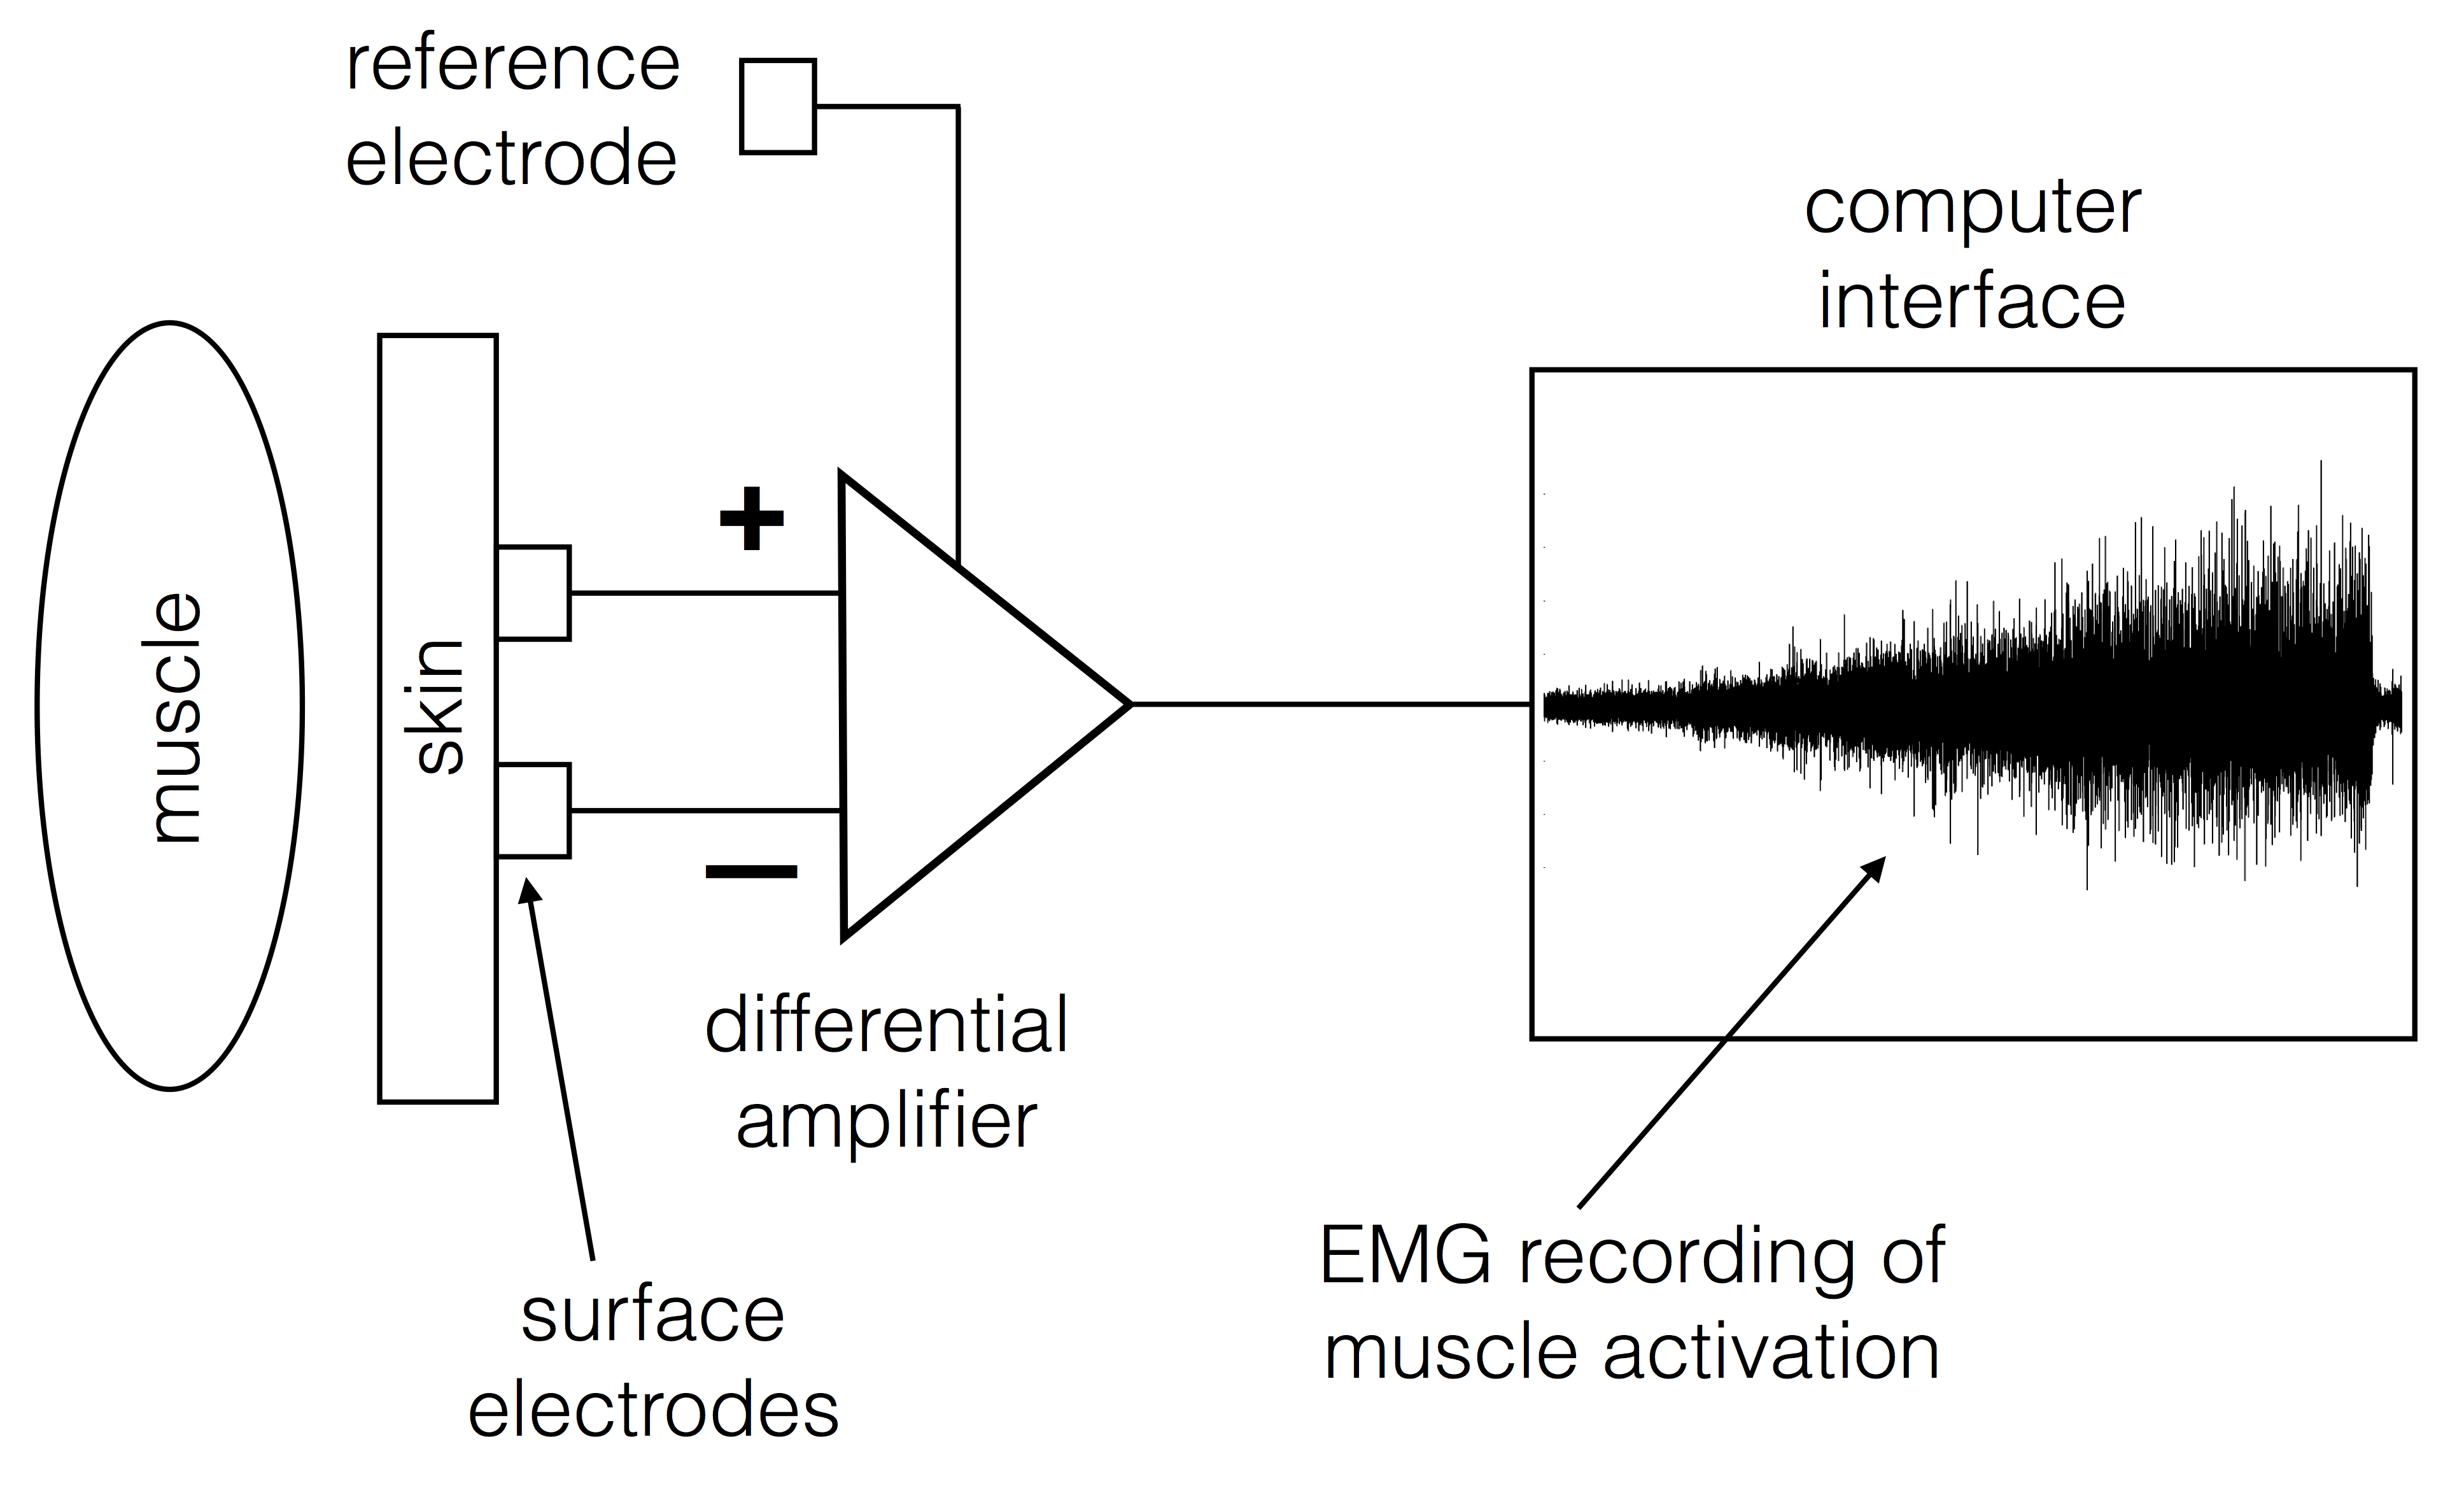
\includegraphics[width=0.7\textwidth]{images/emgAmp.png}
\caption{Bipolar EMG recording setup. For simplicity, not all body or recording components are shown. Image credit: Erin C. McKiernan, CC BY}
\label{fig:emg}
\end{figure}

Bipolar surface EMGs can tell us several things about muscle activity \cite{garcia2011surface}. One is the timing of muscle activation and relaxation. Most muscles show very little activity at rest. When activated, we see a noticeable increase in the occurrence of electrical impulses, as shown in Fig. \ref{fig:emg} (right-hand side). When the muscle relaxes, these impulses disappear and we record only the baseline noise. The timing of muscle activity can then be correlated with other measures; for example, in the case of this practical, with the volume of air inhaled and exhaled. We can also, to some extent, estimate the force or effort exerted during a contraction. As the subject increases the force of contraction, we see an increase in both the frequency of electrical impulses and the signal amplitude. These changes result from two factors: (1) a higher frequency of firing in already active motor units, and (2) the recruitment of additional motor units. Remember, we are recording the activity of multiple motor units. With increasing contraction force, more motor units are recruited and begin to fire, their activity sums, and contributes to the frequency and amplitude increases.

\subsection*{Study questions} 
\begin{enumerate}
\item Where will you need to place the electrodes to record EMGs from the primary inspiratory muscles? Draw the location of the muscles and the electrode placement.
\item Where will you need to place the electrodes to record EMGs from accessory inspiratory or expiratory muscles? Draw the location of the muscles and the electrode placement.
\item Will you be able to record from all muscles groups? Why, or why not? 
\item Which muscles will likely give you the best recordings for each type of respiration? Why?
\item How will you know if you have correctly placed the electrodes?
\end{enumerate}

\subsection*{Pressure-volume relationships during respiration}

The activation and relaxation of the respiratory muscles causes the volume of the lungs to increase or decrease, as described above. These volume changes, in turn, cause pressure changes according to Boyle's Law, which states that the pressure of a gas is inversely proportional to its volume in a closed system. In other words, as the volume increases, the pressure decreases, and vice versa (Fig. \ref{fig:boyle}).

\begin{figure}[h!]
\centering
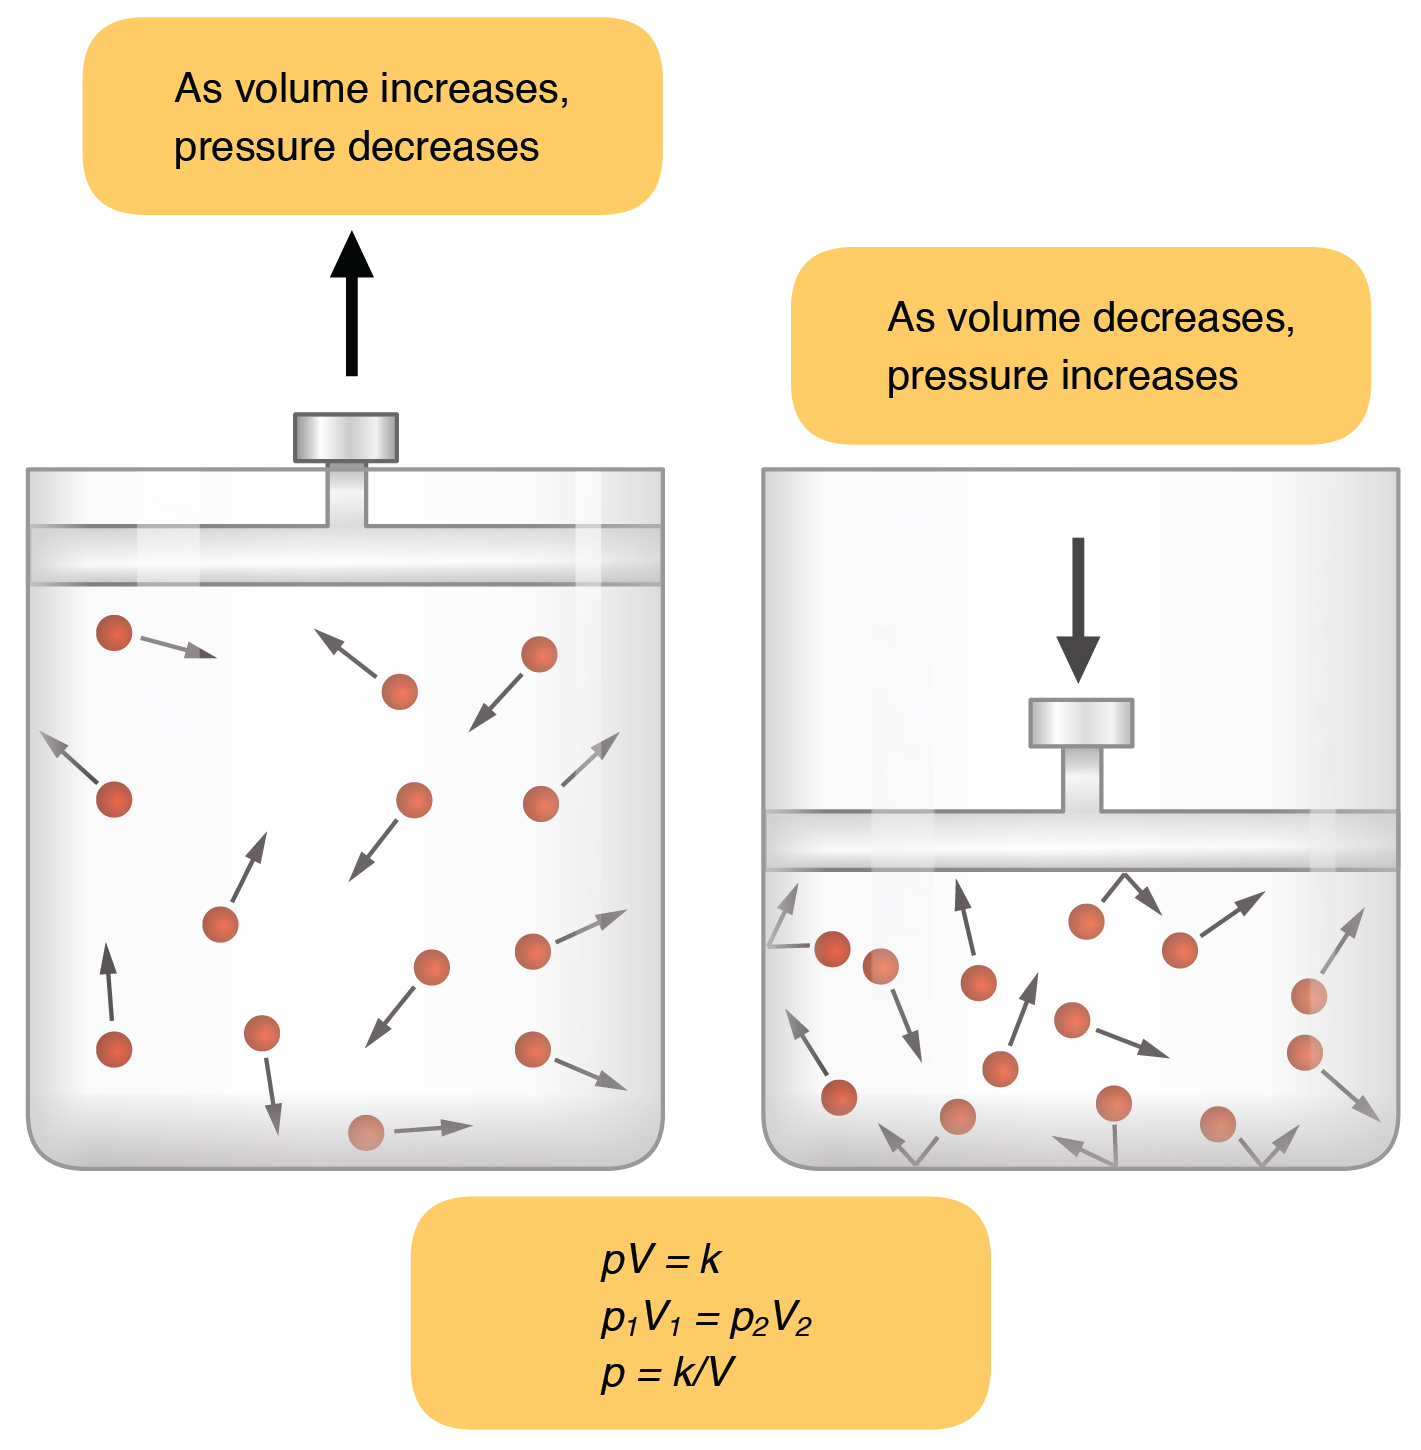
\includegraphics[width=0.6\textwidth]{images/Boyles_Law.jpg}
\caption{Schematic representation of Boyle's Law, where p is pressure, v is volume, and k is a constant. Image credit: OpenStax CNX \cite{openStax2016resp}, CC BY.}
\label{fig:boyle}
\end{figure}

Analogous to Ohm's Law for current flow, airflow is proportional to the pressure gradient \cite{sanchez2010respiratory}:

\begin{equation}
Q= \frac{P_1 - P_2}{R}
\label{eq:ohmFlow}
\end{equation},

where $\dot{Q}$ is the flow rate, $P_1$ and $P_2$ are the pressures at the beginning and end points of a pathway, and $R$ is the resistance of the path. In the respiratory system, the pressures of interest are the atmospheric ($P_{atm}$) and the alveolar ($P_{alv}$) pressures, and the resistance is that of the airways ($R_{aw}$) \cite{sanchez2010respiratory}. Thus, we can rewrite Equation \ref{eq:ohmFlow} as,

\begin{equation}
Q= \frac{P_{atm} - P_{alv}}{R_{aw}}.
\label{eq:ohmFlowResp}
\end{equation},

Air flows down a pressure gradient from an area of high to low pressure. Therefore, during inspiration, the diaphragm and the external intercostals act to increase the volume of the lungs, $P_{alv}$ drops below $P_{atm}$, and air flows into the lungs (Fig. \ref{fig:pressures}a). During exhalation, the elastic recoil of the thoracic cavity and lungs causes their volume to decrease, the $P_{alv}$ rises above $P_{atm}$, and air flow outs of the lungs (Fig. \ref{fig:pressures}b).  

\begin{figure}[h!]
\begin{minipage}{.5\textwidth}
\centering
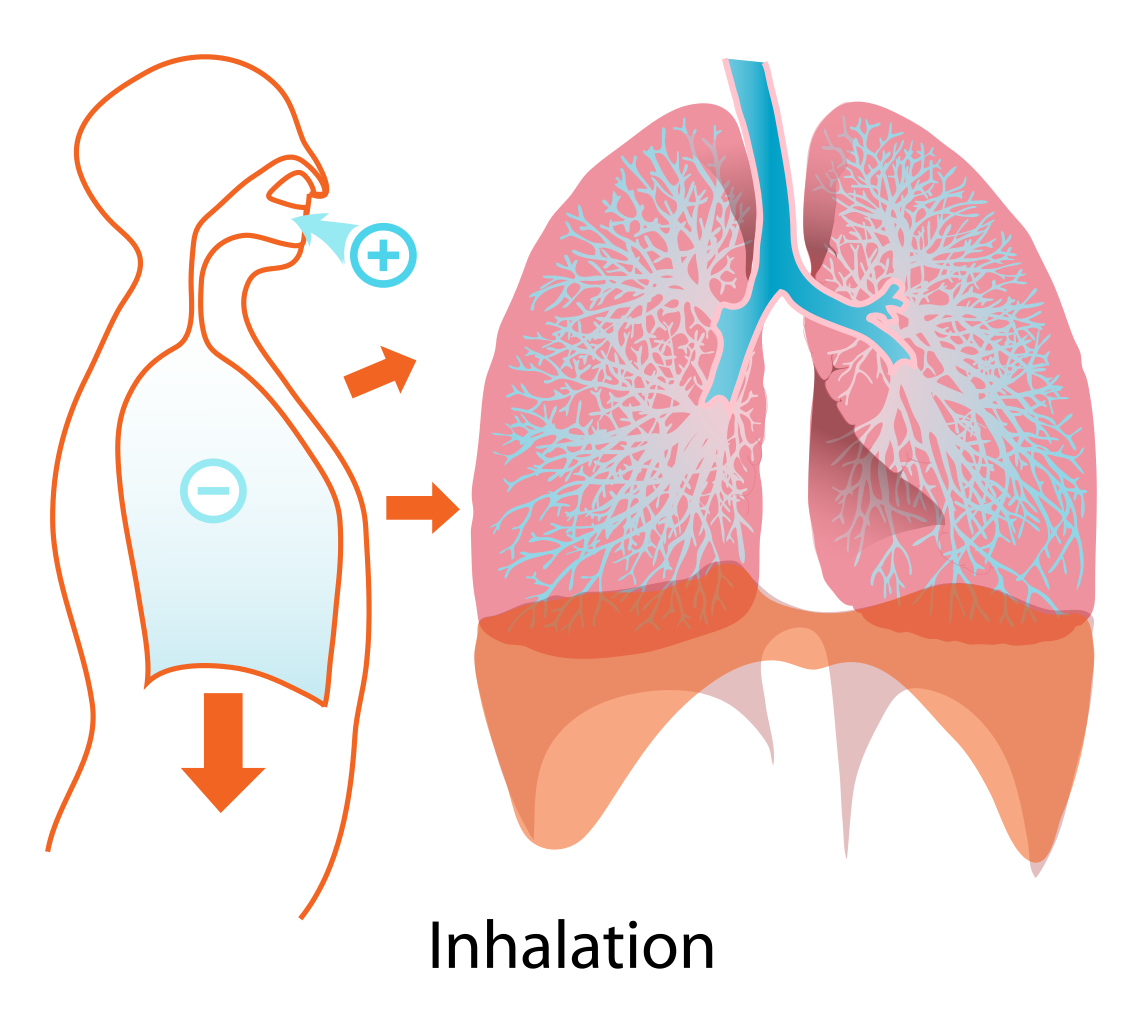
\includegraphics[width=0.9\textwidth]{images/inhalation.png}
\end{minipage}%
\begin{minipage}{.5\textwidth}
\centering
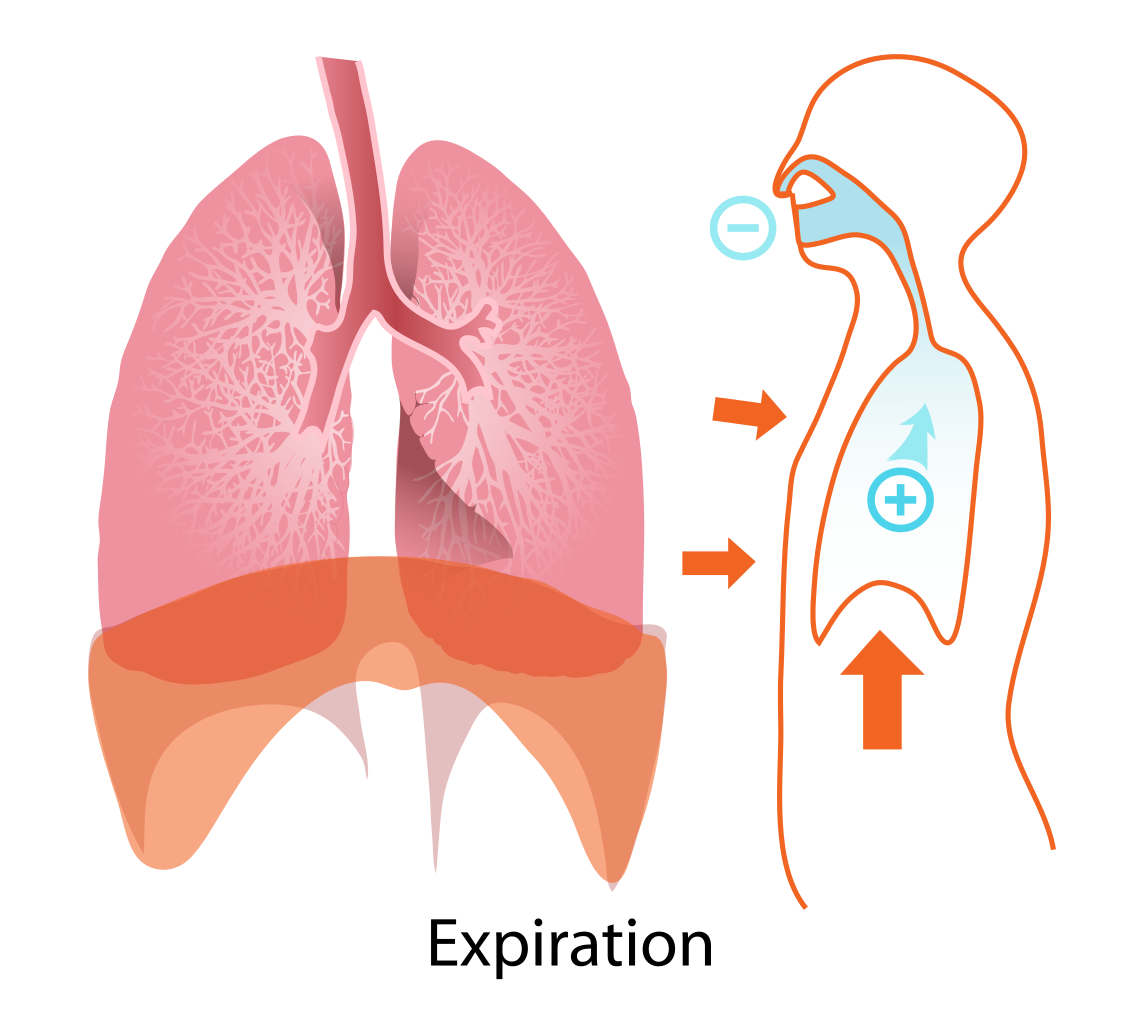
\includegraphics[width=0.9\textwidth]{images/exhalation.png}
\end{minipage}
\caption{The pressure gradient ($P_{alv}-P_{atm}$) determines the flow of air in and out of the lungs. Pressures are shown as relative. During inspiration, intrapulmonary pressure drops below atmospheric (negative versus positive sign). During exhalation, intrapulmonary pressure rises above atmospheric (signs reversed). Image credit: LadyofHats (Mariana Ruiz Villarreal) via Wikimedia Commons, public domain.}
\label{fig:pressures}
\end{figure}

\subsection*{Measuring changes in air volume during respiration - spirometry}

We can measure the volume of air inhaled or exhaled during respiration with the use of a spirometer. There are several different types of spirometer (for review see \cite{schlegelmilch2011pulmonary}). The kind we will use in this practical has a built-in pressure transducer. The subject breathes into a tube and the air then passes through a filter, both of which help to ensure the air flow is laminar. In the center of the device there is a thin mesh screen called a pneumotach that acts as a resistor. Under laminar flow conditions, the pressure drop across a resistor is proportional to the flow rate of a fluid (gas or liquid), as described by Poiseuille's law:

\begin{equation}
Q=\frac{\Delta P \pi r^{4}}{8 l \eta}
\label{eq:presion}
\end{equation},

where Q is the flow rate, $\Delta P$ is the pressure difference between two points, $\eta$ is the fluid viscosity, and $r$ and $l$ are the radius and length of the tube through which flow occurs. 

Thus, as the subject breathes and air moves across the screen, there is a pressure drop that is proportional to the air flow rate. Tubes on either side of the screen transmit these pressures to a transducer, which takes the difference in pressure between the two points (P1-P2), giving us the flow rate. Note that the pressure difference will be positive or negative depending on whether the subject is exhaling or inhaling, respectively. Integrating the flow rate over time then gives us the volume of air exhaled or inhaled.  
\begin{figure}[h!]
\centering
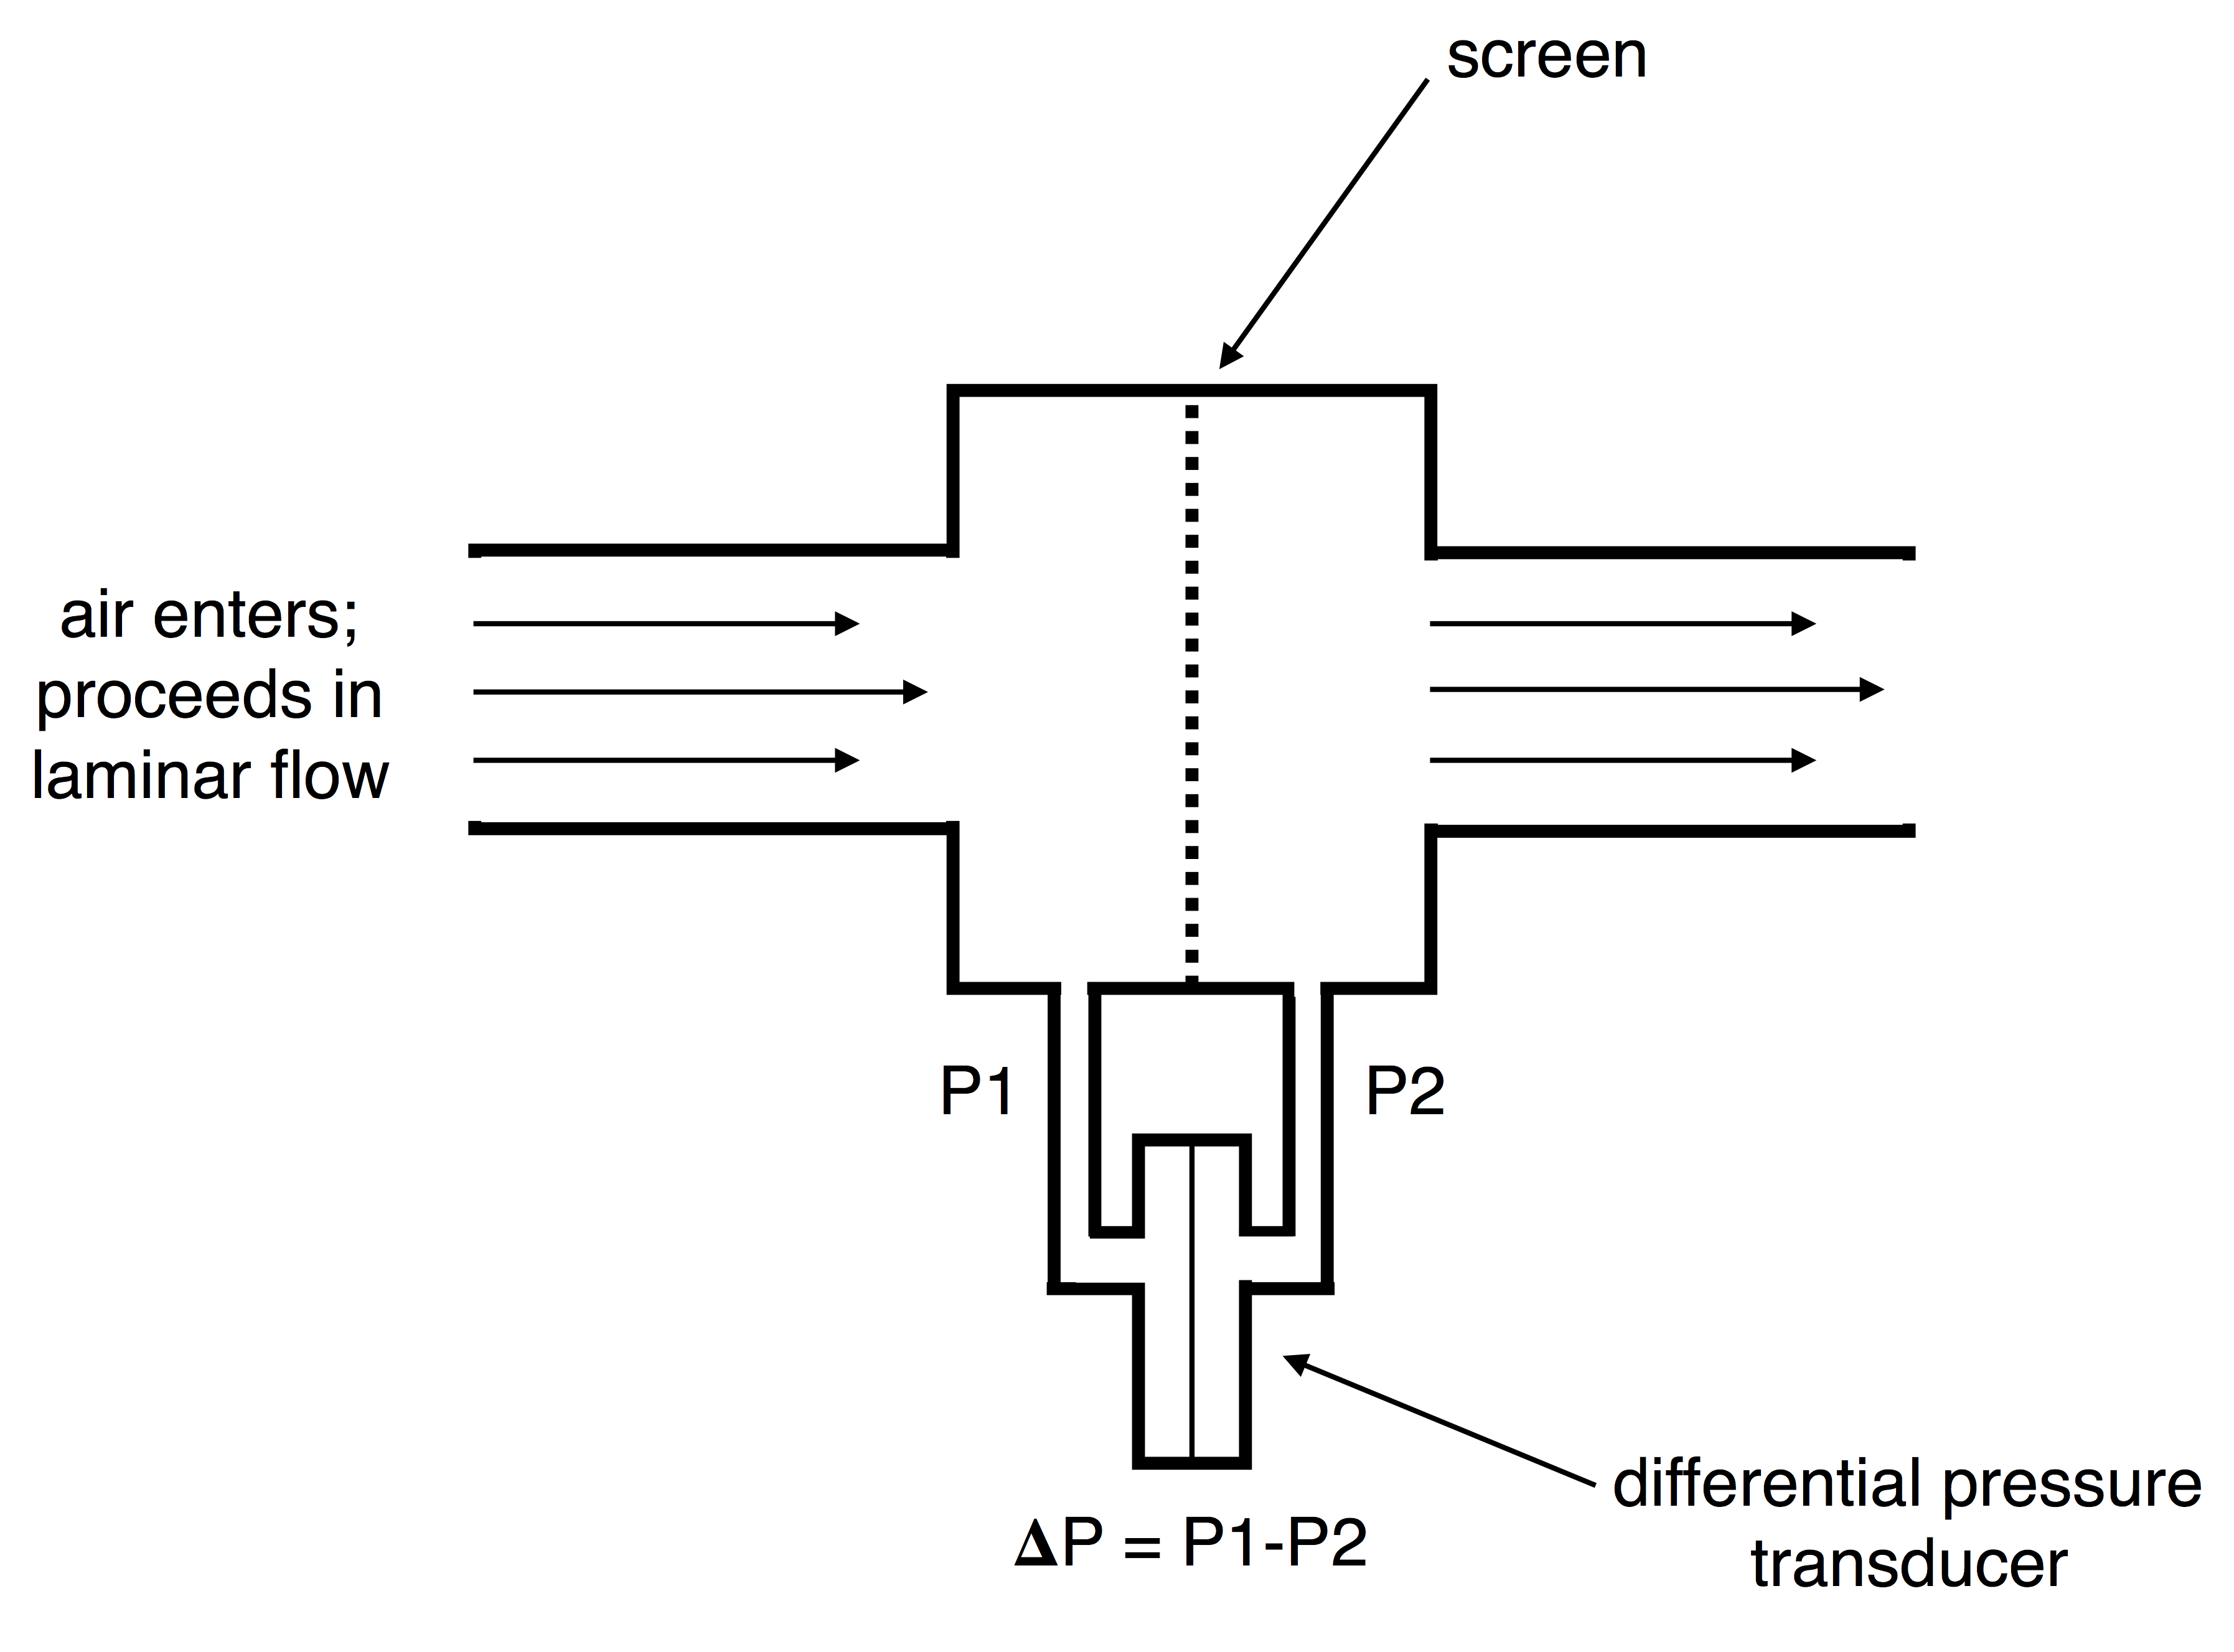
\includegraphics[width=0.7\textwidth]{images/pneumotach.png}
\caption{Schematic of a spirometer which uses a differential pressure transducer. Image credit: Erin C. McKiernan, CC BY.}
\label{fig:pneumotach}
\end{figure}

\subsection*{Pulmonary volumes and capacities}

By analyzing the spirogram we can estimate different pulmonary volumes and capacities (Fig. \ref{fig:volsCaps}) \cite{guyton20006textbook,openStax2016resp}. The 3 volumes and 2 capacities that can be measured with spirometry are:

\begin{itemize}
\item \textbf{tidal volume (TV)}: volume of air inhaled and exhaled under normal, resting conditions
\item \textbf{inspiratory reserve volume (IRV)}: additional volume of air that can be inhaled beyond tidal volume when maximum inspiratory force is made
\item \textbf{expiratory reserve volume (ERV)}: additional volume of air that can be exhaled beyond tidal volume when maximum expiratory force is made
\item \textbf{inspiratory capacity (IC)}: the sum of IRV and TV, i.e the total amount of air a person can breathe in
\item \textbf{vital capacity (VC)}: the sum of IRV, TV, and ERV; or, the sum of IC and ERV, i.e. the maximum volume of air that can be forcefully exhaled and inhaling with maximum force
\end{itemize}

The volume of air remaining in the lungs after maximum exhalation, called the residual volume, cannot be measured with spirometry \cite{guyton20006textbook}. Because of the contribution of this volume to the functional residual capacity (FRC) and the total lung capacity (TLC), these capacities are also not measurable with this technique. 

The measurable volumes and capacities can vary up to 25\% between men and women \cite{guyton20006textbook}. These values also vary with age, athletic status, and certain respiratory diseases.

\begin{figure}[h!]
\centering
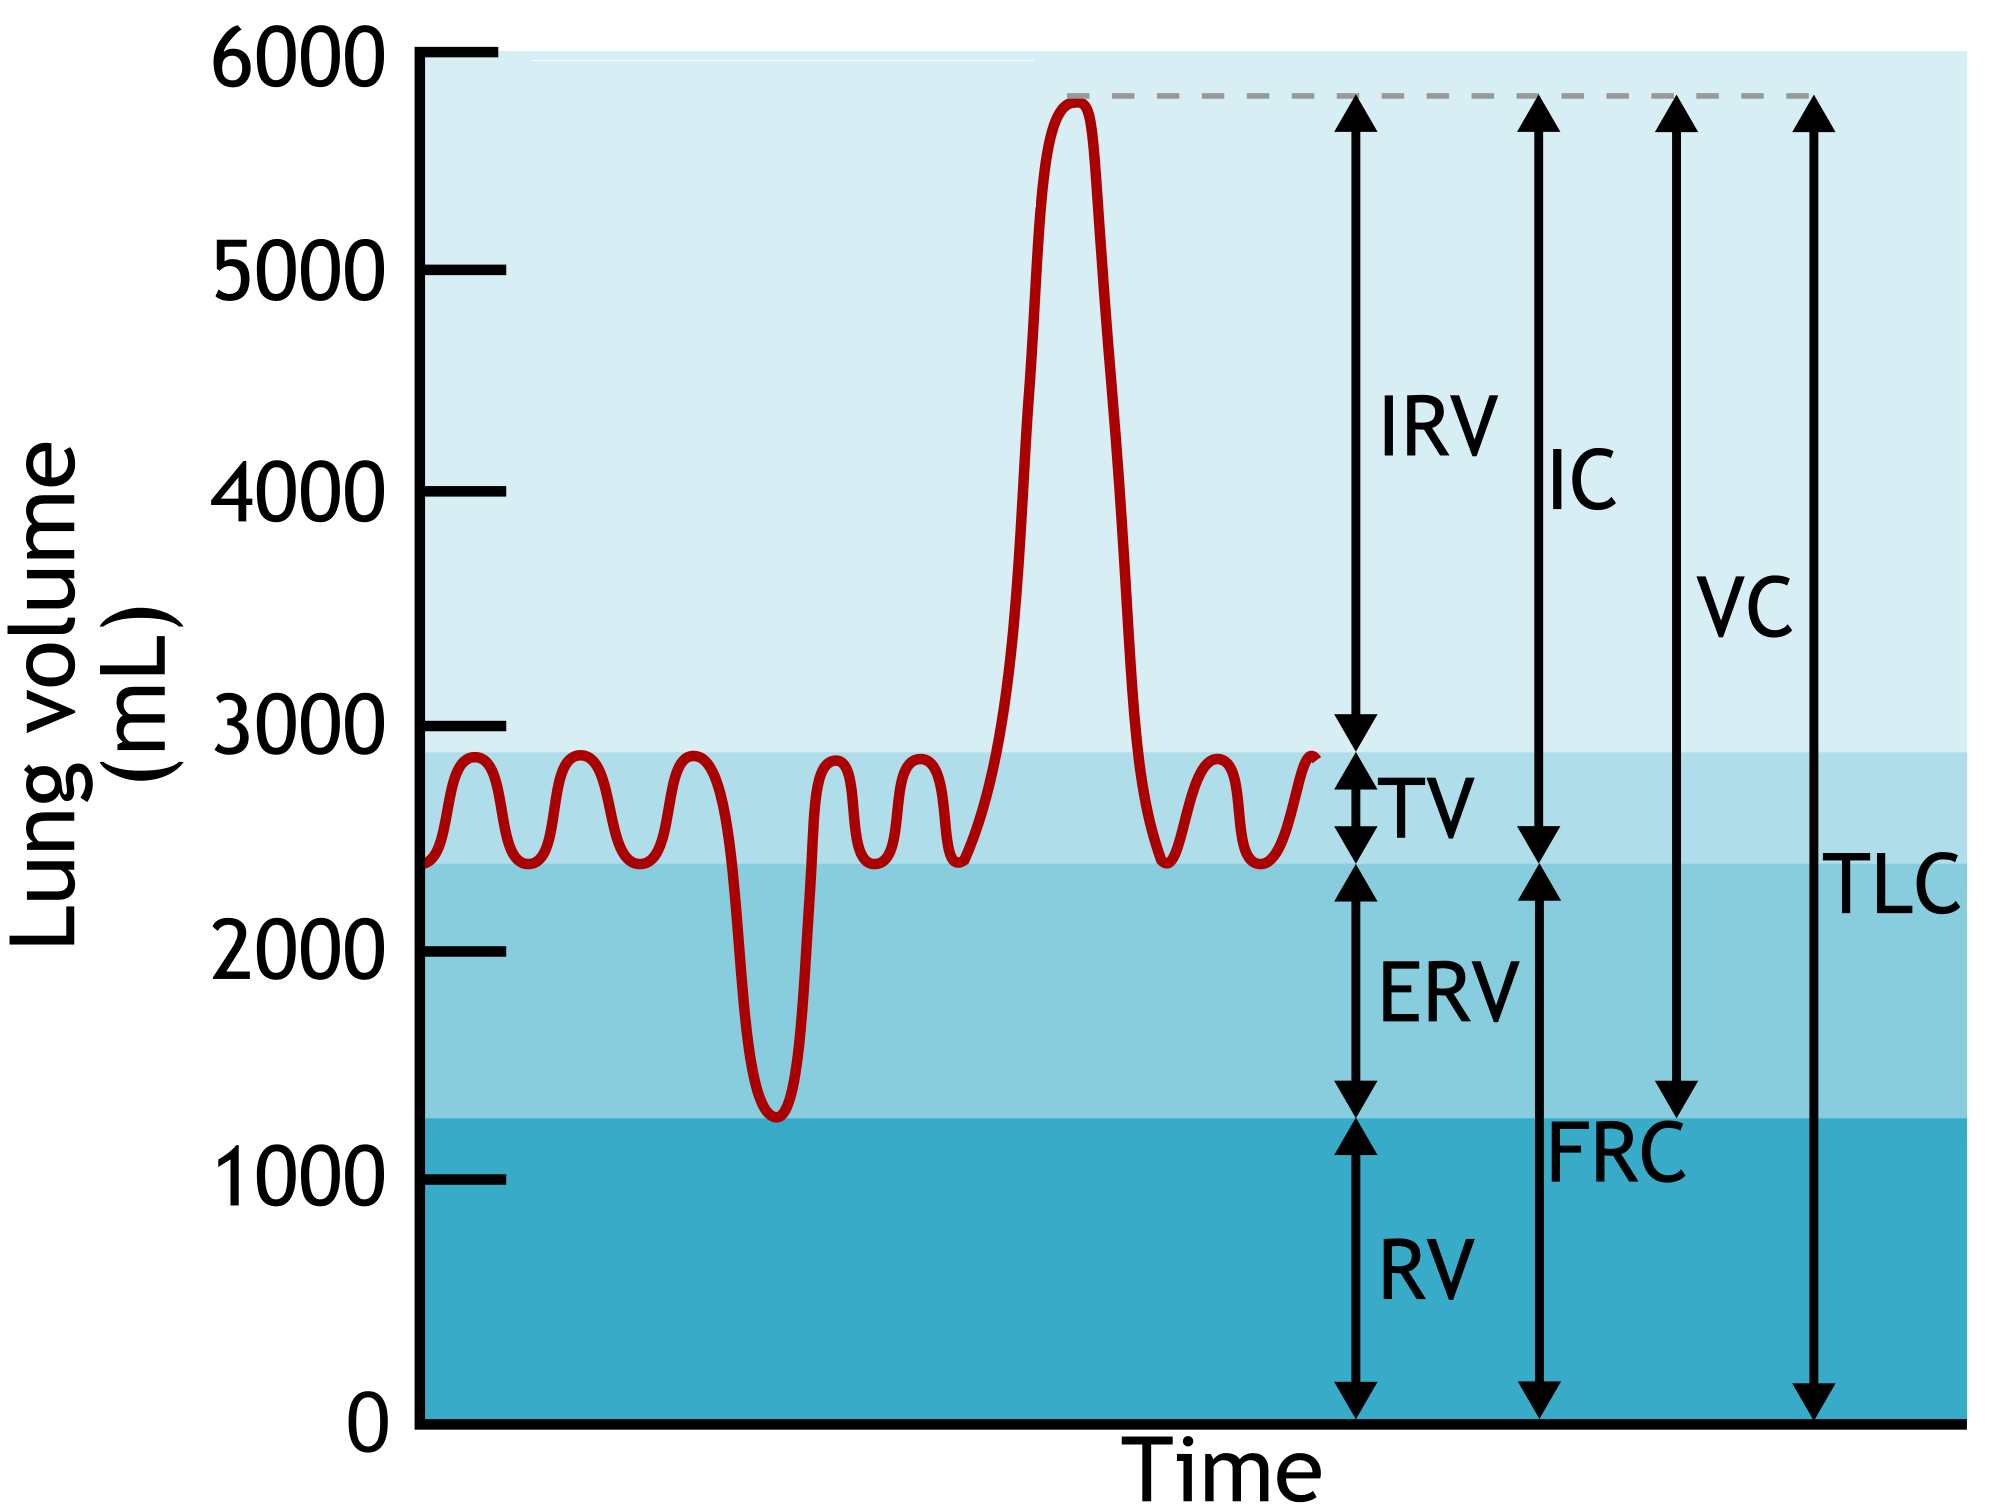
\includegraphics[width=0.8\textwidth]{images/volumesCapacities.png}
\caption{Inspiratory volumes and capacities. Subject takes two normal breathes in and out, followed by normal inspiration then maximum expiration, then two normal breathes again, followed by a maximum insp  Image credit: Michal Komorniczak via Wikimedia Commons, CC BY-SA.}
\label{fig:volsCaps}
\end{figure}

\section*{PROCEDURE}

Before beginning, make sure you have all the necessary equipment and have installed the recording software on your computer or smartphone. The following steps will guide you in assembling the equipment and carrying out recordings.

\subsection*{1. Assemble the spirometer}

If your spirometer is newly purchased, you will need to perform all the following steps to assemble the device. If you have used the device previously, only steps ? and ? are necessary.

\vspace{0.2cm}

\begin{enumerate}
\item Push in the two latches at the top of the handle so that they move outwards 
\item Insert the flow head into the handle and push the latches in to lock in place 	
\item Attach the bacterial filter to the side of the flow head marked `inlet'
\item Attached the disposable mouthpiece to the end of the filter
\end{enumerate}

\vspace{0.2cm}

When your spirometer is correctly assembled, it should look like this:

\vspace{0.2cm}

\begin{figure}[h!]
\begin{center}
\begin{minipage}{.5\textwidth}
\centering
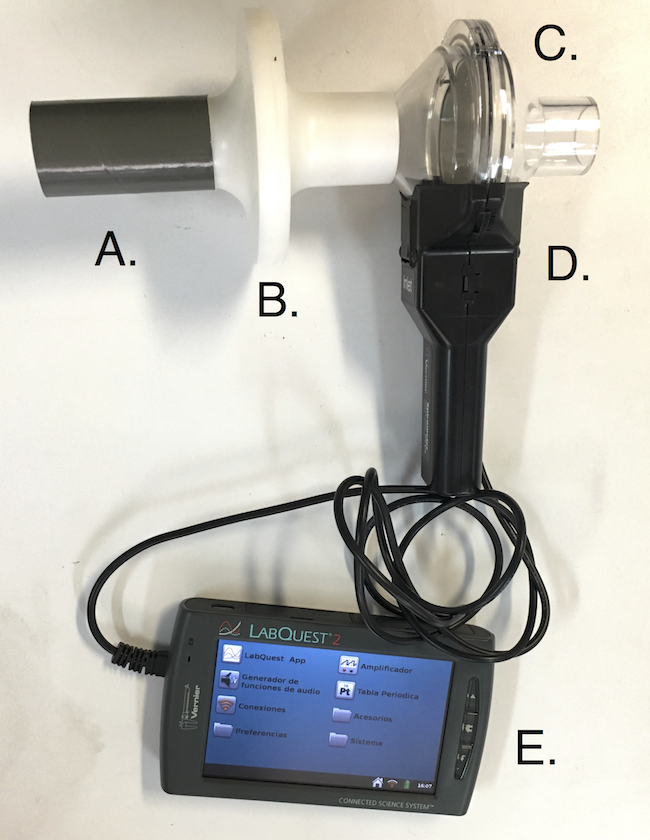
\includegraphics[width=0.9\textwidth]{images/spirometer.png}
\end{minipage}%
\begin{minipage}{.43\textwidth}
\centering
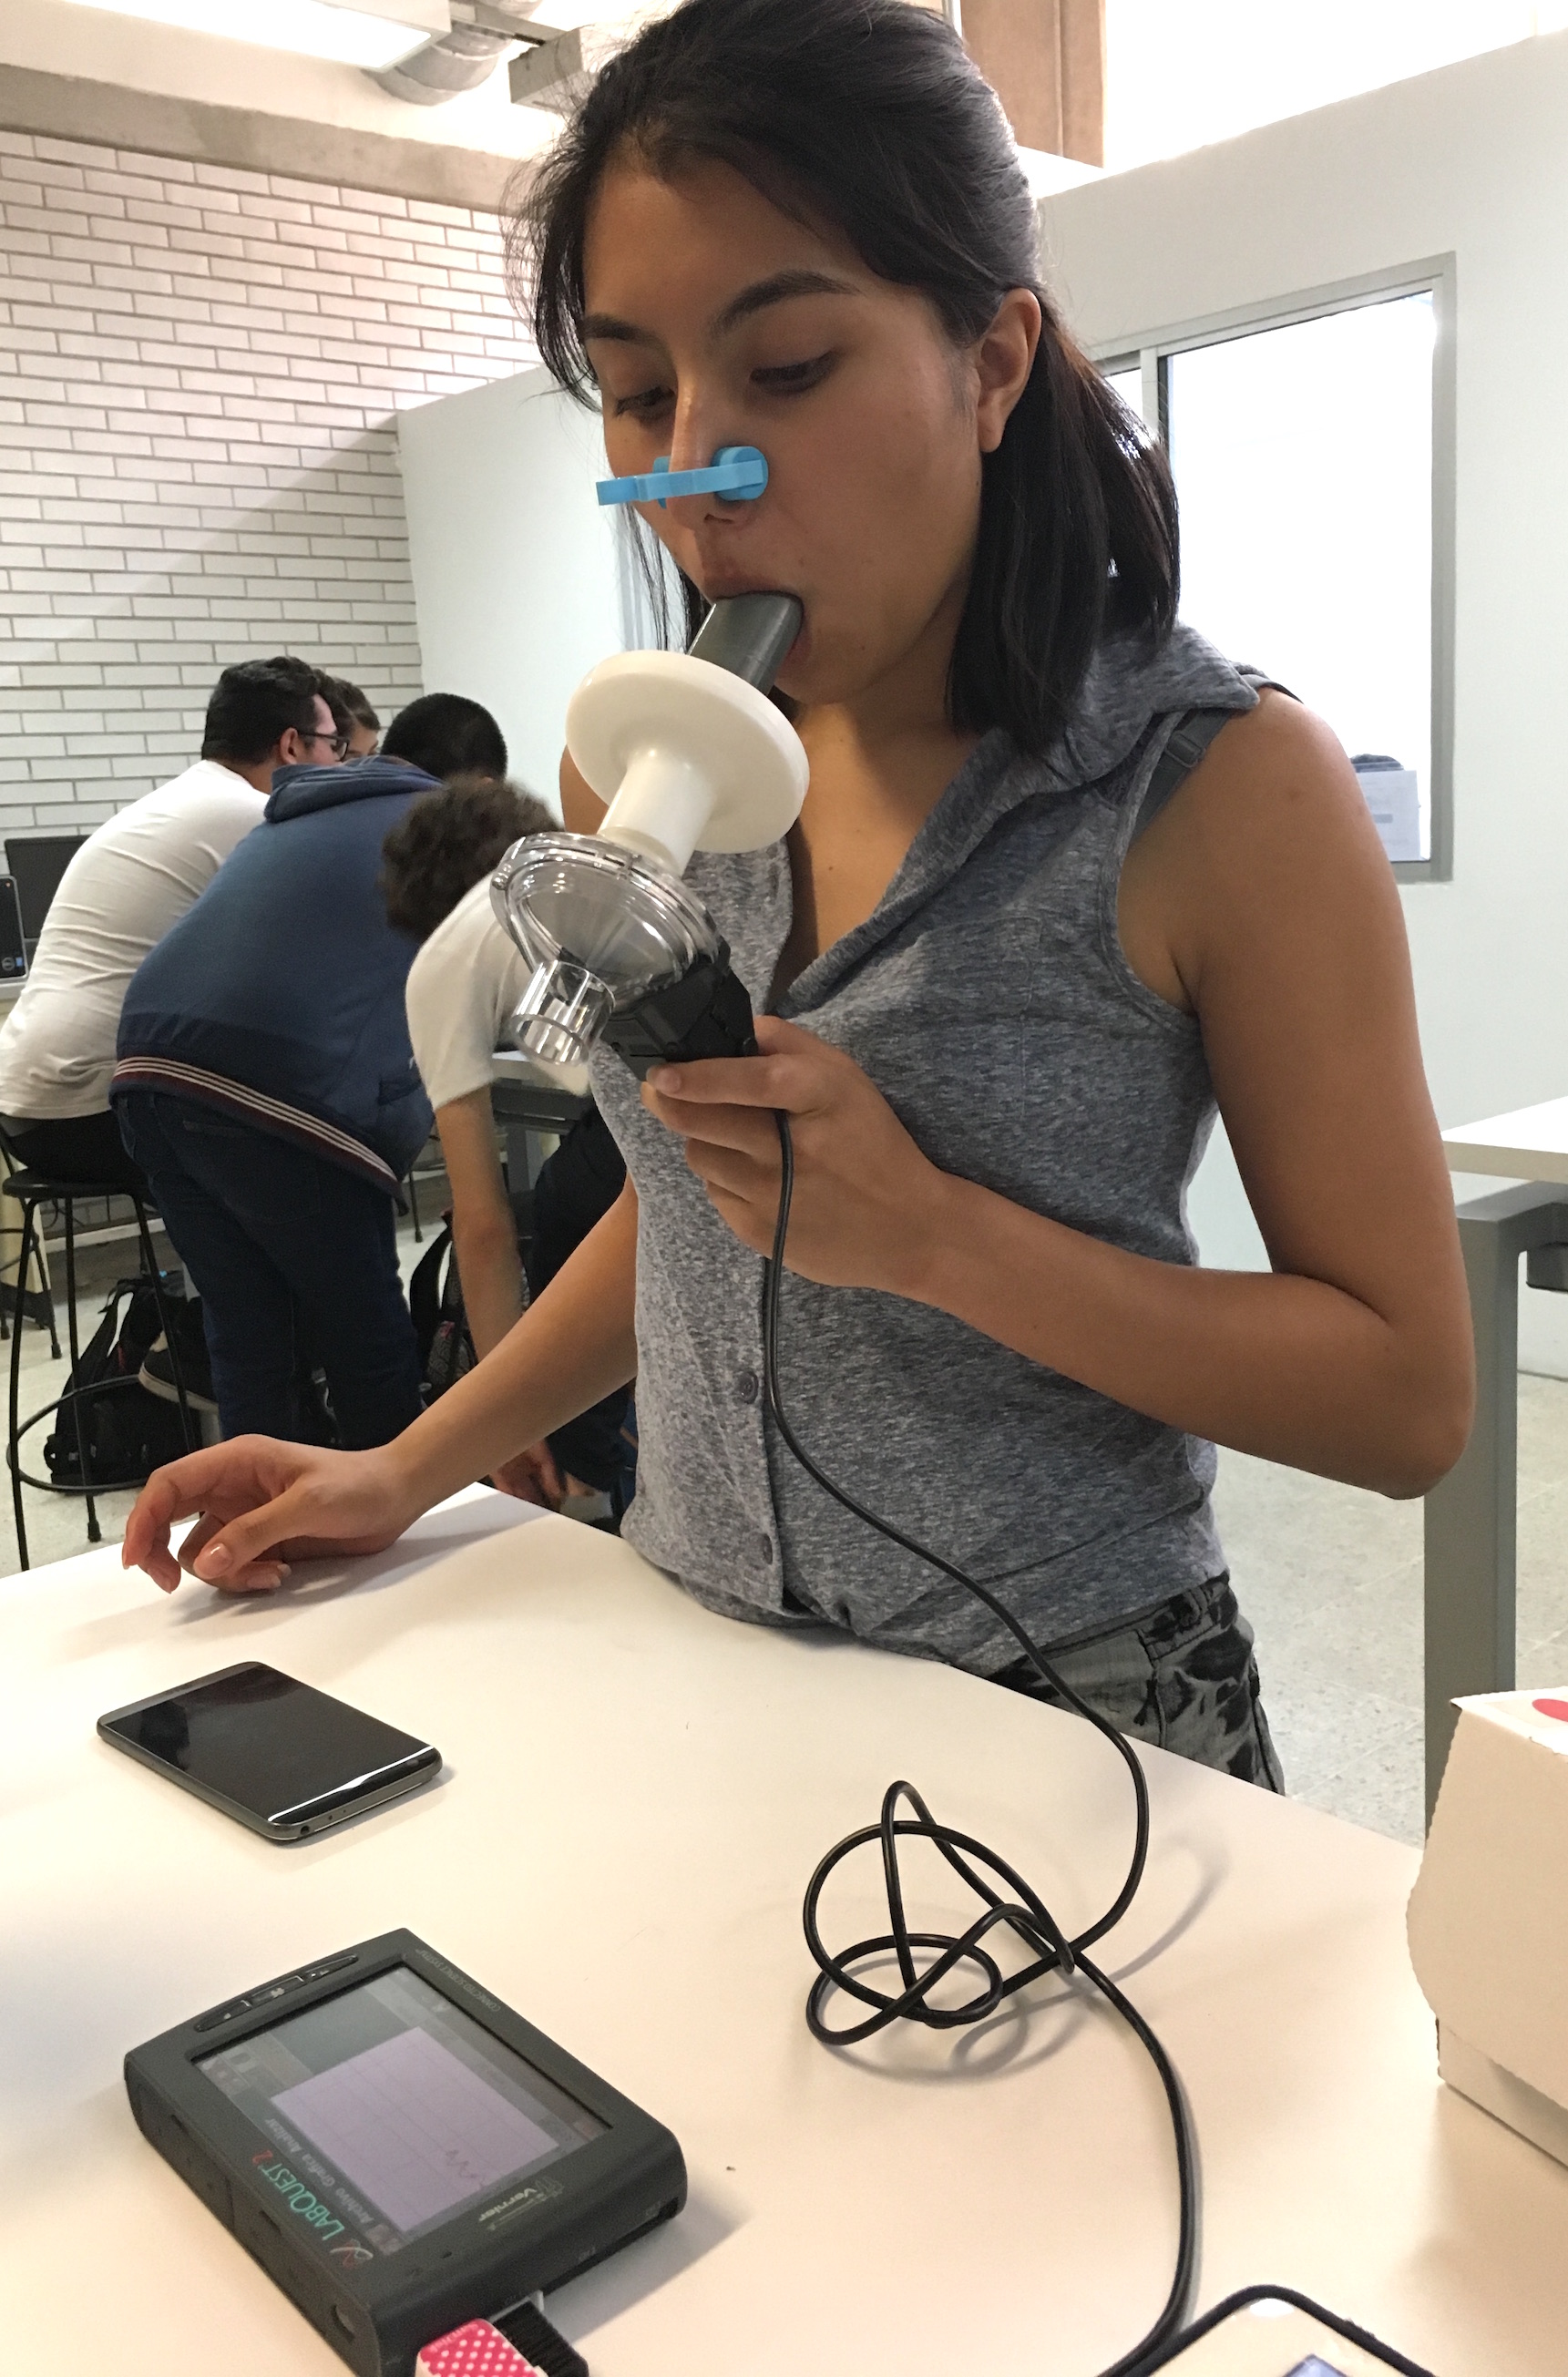
\includegraphics[width=0.9\textwidth]{images/spiro_breathing.JPG}
\end{minipage}
\end{center}
\caption{Left: Fully assembled spirometer, showing disposable breathing tube (A.), bacterial filter (B.), plastic encasing containing screen (C.), plastic encasing containing differential pressure transducer (D.), and LabQuest interface (E.). Right: Student using spirometer during practical. Image credit: ?, CC BY}
\label{fig:spirAssembly}
\end{figure}

\subsection*{2. Test the spirometer}

\begin{enumerate}
\item Connect the spirometer to the interface (computer or LabQuest 2 portable device)
\item Open the LabQuest software and explore the different functions
\item Tell the subject to inhale and exhale into the spirometer mouthpiece
\item Verify that the interface is showing the corresponding changes in volume as subject breathes
\item Try saving and exporting a data file (use txt format)
\end{enumerate}

\subsection*{3. Setup EMG recordings}

The Backyard Brains Muscle SpikerBox comes fully assembled and ready to record. All you have to do is connect the battery, cables, and electrodes.

\vspace{0.2cm}

\begin{enumerate}
\item Connect the 9V battery to its terminals on the Muscle SpikerBox
\item Connect the black/blue or green cable to the corresponding computer or smartphone port on the Muscle SpikerBox; note that the smartphone cable is directional, make sure you have the correct end inserted into the device
\item Connect the other end of the black/blue or green cable to your computer or smartphone
\item Connect the orange cable to its corresponding port on the Muscle SpikerBox
\item Place the surface electrodes over the muscle of interest approximately ? cm apart and oriented parallel to the muscle fibers
\item Connect each of the red aligator clips on the end of the orange cable to one of the surface electrodes; make sure the metal clips do not touch and try to avoid entangling the cables 
\item Hold the black aligator clip (reference) in your hand, or connect it to another surface electrode on the back of your hand or some other area away from the recording site

\vspace{0.2cm}

\begin{figure}[h!]
\begin{center}
\begin{minipage}{.55\textwidth}
\centering
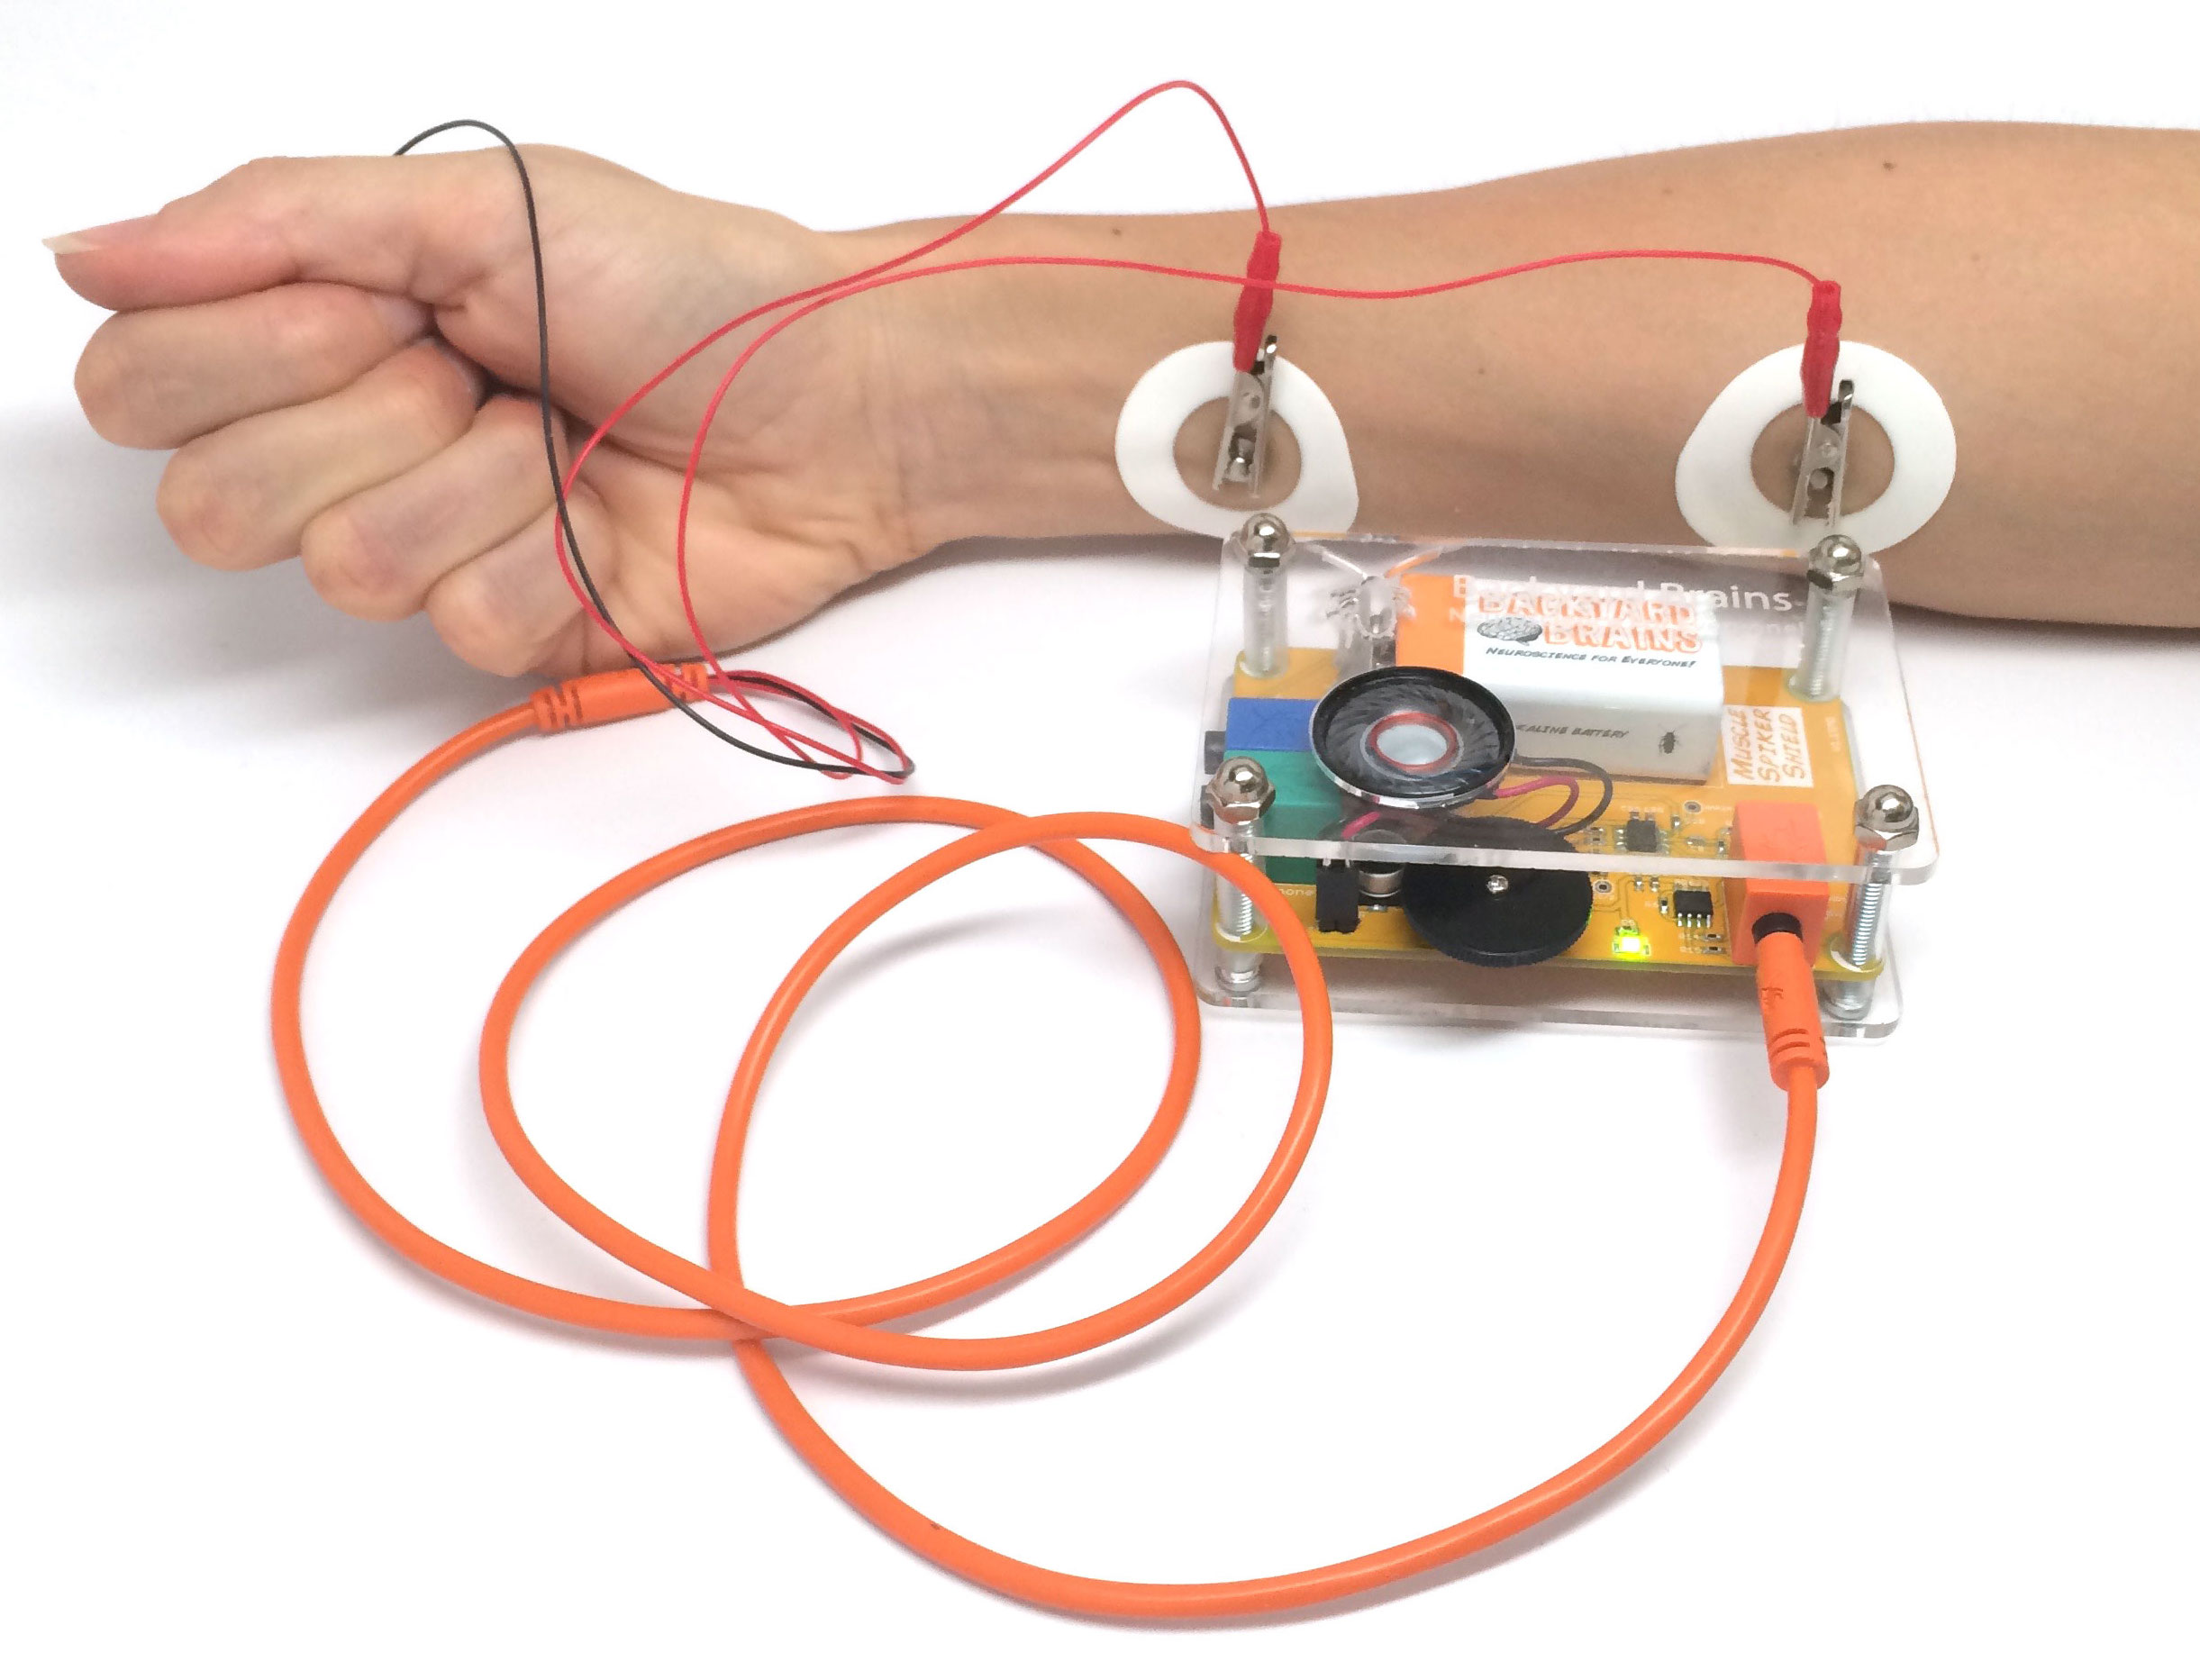
\includegraphics[width=0.9\textwidth]{images/muscleSpikerBox.jpg}
\end{minipage}%
\begin{minipage}{.4\textwidth}
\centering
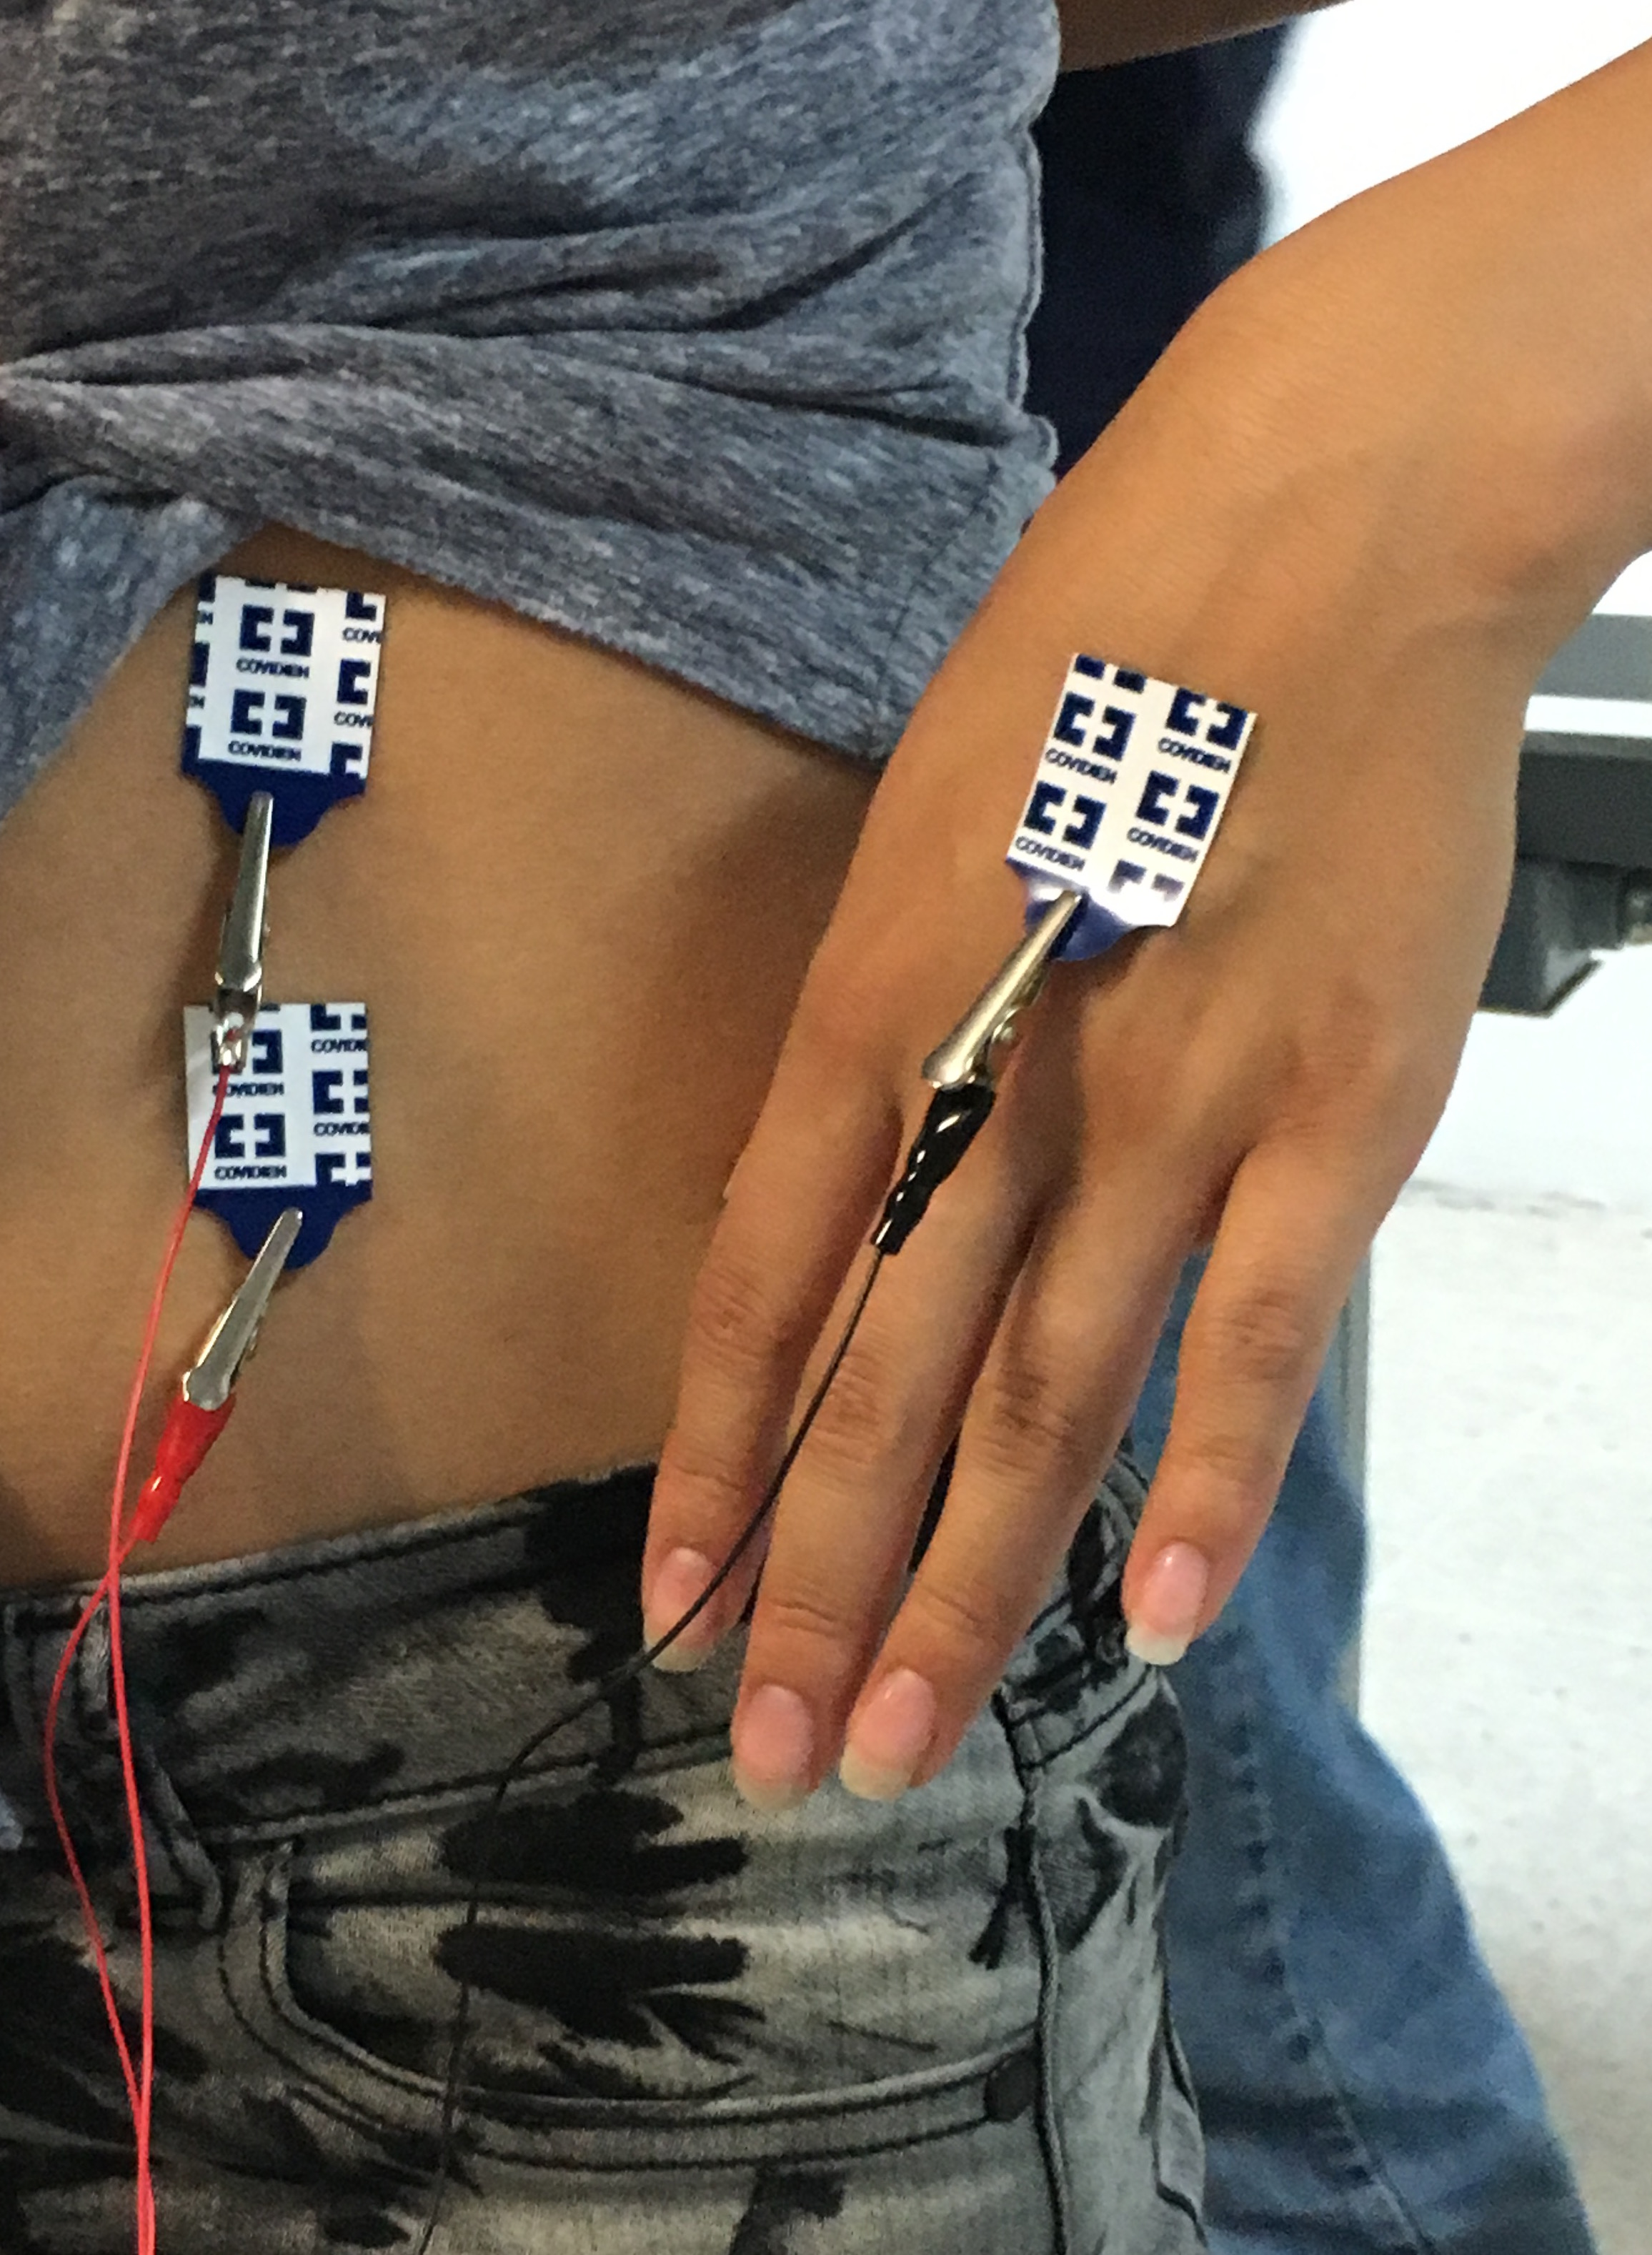
\includegraphics[width=0.8\textwidth]{images/electrodeAb.JPG}
\end{minipage}
\end{center}
\caption{\textit{Left}: EMG setup with electrodes connected to Muscle SpikerBox. (Connection to computer or smartphone not shown.) Image credit: Backyard Brains, CC BY SA. \textit{Right}: Surface electrodes placed to record from the rectus abdominus muscle during forced expiration. Image credit: ?, CC BY}
\label{fig:spirAssembly}
\end{figure}

\item To improve the EMG signal, the area where the electrodes will be placed can be cleaned with alcohol prior to placement; wait until the area is dry to place the electrodes
\item Electrode gel can be placed to improve conduction but is often not necessary
\item To avoid noise artifacts, ensure that no clothing is touching the electrodes or brushing against the cables during recording
\end{enumerate}
 
\subsection*{4. Test EMG recordings}

\begin{enumerate}
\item Turn on the Muscle SpikerBox by rotating the black wheel switch on the side, a green light should turn on; note that electrodes should be connected before turning on the device and disconnected only after the device is turned off to avoid a nasty noise!
\item Open the Backyard Brains recording software and explore the controls and settings (for more info on software use, see \cite{spikeRecorder})

\begin{figure}[h!]
\centering
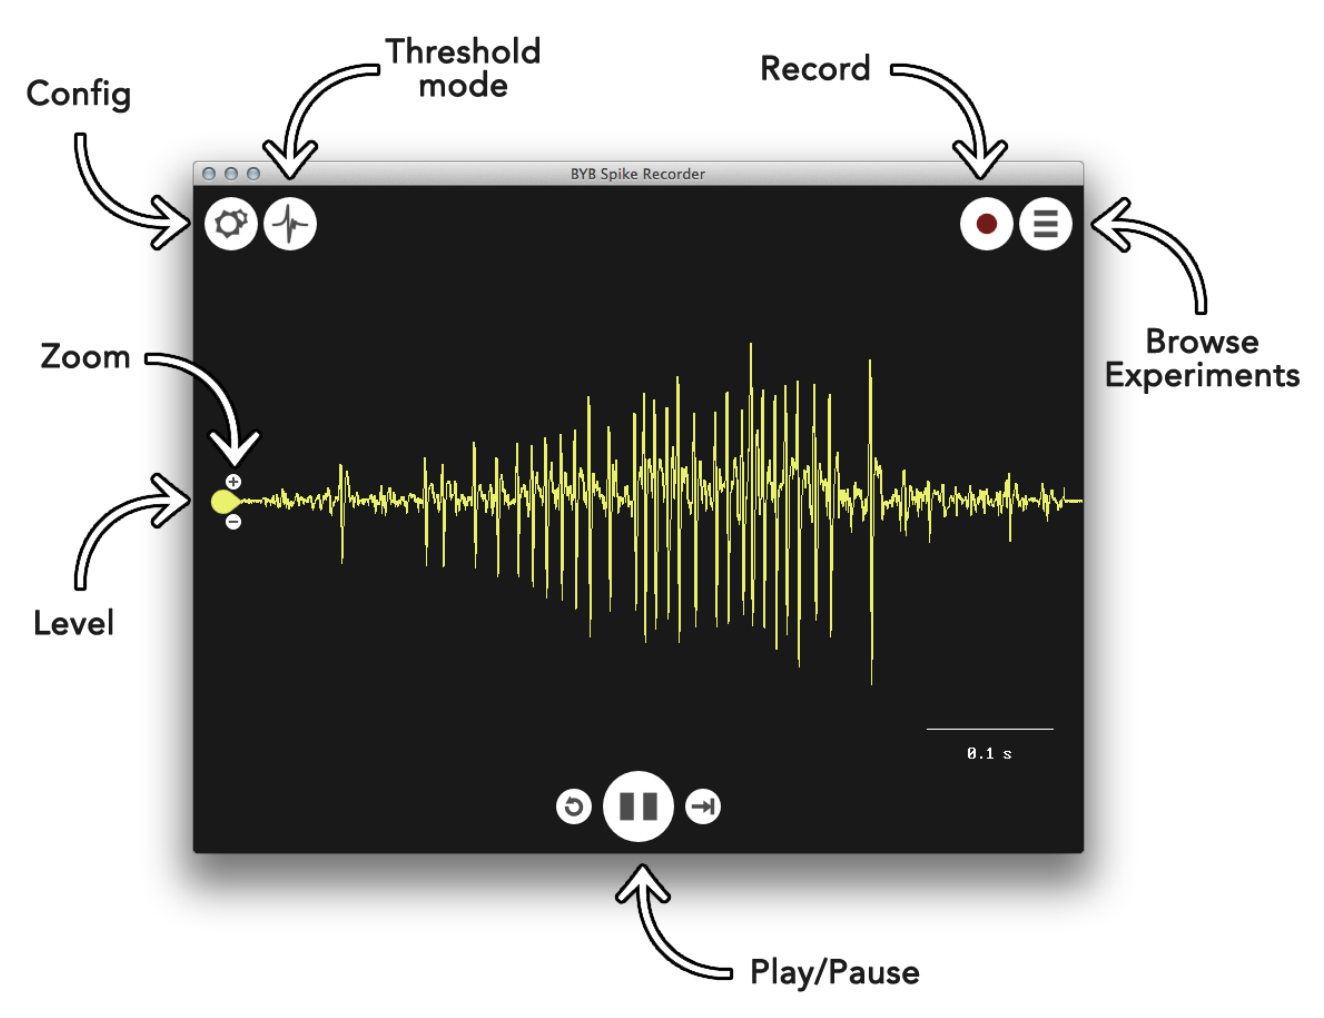
\includegraphics[width=0.8\textwidth]{images/BBrecorder.png}
\caption{Recording software interface. Image credit: Backyard Brains, CC BY SA}
\label{fig:recorder}
\end{figure}

\item Snap your fingers near the recording device; if you see a corresponding artifact on the screen, this means you are recording only audio; to begin recording muscle activity, adjust the settings by pressing the `Config' button (Fig. \ref{fig:recorder}) (see \cite{spikeRecorder} for more details)
\item Ask the subject to briefly contract and relax the muscle of interest 
\item Verify that electric potentials are observed during the contraction; check your signal to noise rati; if the signal is too small, you can adjust the gain by turning the wheel switch to the right
\item Try saving a recording to your computer or smartphone (format will be .wav)
\end{enumerate}

\subsection*{5. Collect your data}

\begin{enumerate}
\item Make sure EMG is ready to record, and the subject has the spirometer in hand
\item Place the blue clip over the nose of the subject; if they find it uncomfortable, simply ask them to hold their nose during the exercise
\item Instruct the subject that when the recording begins, they will perform the following sequence:
	\begin{itemize}
	\item two normal breaths
    \item normal inhalation followed by a maximal forced exhalation
    \item two normal breaths
    \item maximal forced inhalation followed by normal exhalation
    \item two normal breaths
    \item maximal forced inhalation followed by maximal forced exhalation
    \item two normal breaths
	\end{itemize}
\item You can put an image like that seen in Fig. \ref{fig:volsCaps} in front of the subject and instruct them verbally to help them remember the sequence
\item Since you are recording on two different devices, you must do your best to manually synchronize the recordings; have one person in charge of pressing record on the EMG and another in charge of the spirometer recording
\item Count to 3 and have the two people press `record' on the different devices at the same time
\item At the end of the sequence, count to 3 again and have the two people end the recordings at the same time
\item Save the data to your computer or smartphone; if working on the LabQuest2, you can save the data to a USB memory stick 
\item EMGs should be saved and exported in .wav and spirograms in .txt formats for analysis
\item If gathering data from additional subjects, clean out the spirometer with alcohol wipes and replace the disposable mouthpiece with a new one before proceeding
\end{enumerate}

%\section*{MORE INFORMATION}
%This document only includes background information and methods necessary to understand and carry out the practical. To see sample results from this practical, please refer to document ?. To learn how to open and analyze the EMG and spirogram files, please refer to document ?. All materials associated with this practical are openly licensed for reuse and available online at ?.

\section*{ACKNOWLEDGMENTS}
This work was supported by UNAM-DGAPA-PAPIME PE213817 and PE213219.

% BIBLIOGRAPHY
\renewcommand\refname{REFERENCES}
\renewcommand{\markboth}[2]{}%
\begin{footnotesize}
\bibliography{resp}
\end{footnotesize}


\end{document}
